\documentclass[conference]{IEEEtran}
\IEEEoverridecommandlockouts
% The preceding line is only needed to identify funding in the first footnote. If that is unneeded, please comment it out.
\usepackage{cite}
\usepackage{amsmath,amssymb,amsfonts}
\usepackage{algorithmic}
\usepackage{graphicx}
\usepackage{textcomp}
\usepackage{xcolor}
\def\BibTeX{{\rm B\kern-.05em{\sc i\kern-.025em b}\kern-.08em
    T\kern-.1667em\lower.7ex\hbox{E}\kern-.125emX}}
\ifCLASSOPTIONcompsoc
    \usepackage[caption=false, font=normalsize, labelfont=sf, textfont=sf]{subfig}
\else
\usepackage[caption=false, font=footnotesize]{subfig}
\fi

\begin{document}

\title{The performance of algorithms in crop yield forecasting}

\author{\IEEEauthorblockN{1\textsuperscript{st} Given Name Surname}
\IEEEauthorblockA{\textit{dept. name of organization (of Aff.)} \\
\textit{name of organization (of Aff.)}\\
City, Country \\
email address or ORCID}
\and
\IEEEauthorblockN{2\textsuperscript{nd} Given Name Surname}
\IEEEauthorblockA{\textit{dept. name of organization (of Aff.)} \\
\textit{name of organization (of Aff.)}\\
City, Country \\
email address or ORCID}
\and
\IEEEauthorblockN{3\textsuperscript{rd} Given Name Surname}
\IEEEauthorblockA{\textit{dept. name of organization (of Aff.)} \\
\textit{name of organization (of Aff.)}\\
City, Country \\
email address or ORCID}
\and
\IEEEauthorblockN{4\textsuperscript{th} Given Name Surname}
\IEEEauthorblockA{\textit{dept. name of organization (of Aff.)} \\
\textit{name of organization (of Aff.)}\\
City, Country \\
email address or ORCID}
\and
\IEEEauthorblockN{5\textsuperscript{th} Given Name Surname}
\IEEEauthorblockA{\textit{dept. name of organization (of Aff.)} \\
\textit{name of organization (of Aff.)}\\
City, Country \\
email address or ORCID}
\and
\IEEEauthorblockN{6\textsuperscript{th} Given Name Surname}
\IEEEauthorblockA{\textit{dept. name of organization (of Aff.)} \\
\textit{name of organization (of Aff.)}\\
City, Country \\
email address or ORCID}
}

\maketitle

\begin{abstract}
  With the rapid growth of the population and the development of economy, the demand for food production by people all over the world are significantly increasing. However, under the circumstance that the cultivated land area has not expanded in recent ten years, a feasible way to raise the total production of crops is to improve the yield per unit area. This requires accurate yield forecasting algorithms by monitoring status of crops to suggest farmers how to cultivate the crops better. To pick out the algorithms with best performance in predicting the agricultural yield, this paper compares several regression algorithms within the current datasets. The experimental results illustrate that random forest and Bi-LSTM model both have high metrics on production predicting and their accuracy reaches 85\% higher after solving the overfitting problem. Therefore, these two algorithms are prior choices to implement crop yield forecasting.
  % 实验的结果还需要改
\end{abstract}

\begin{IEEEkeywords}
  Prediction, Agricultural Yield, Random Forest, LSTM RNN
\end{IEEEkeywords}

\section{Introduction}
  The food issue has always been a hot topic and it directly affects many aspects of people's lives. With the explosive growth of the world population, countries all over the world are exploring methods to grow crops with less natural resource consumption while increasing production under the guarantee of environmental protection. In such situation, the precision and intelligence of agriculture are becoming increasingly important. Therefore, researchers have focused on the collection, combination and processing of external information such as climate, satellites and geography in recent years. Such researches may improve modern agricultural technology and also help increase agricultural yield and quality.

  The forecast of crop yield is an important part of modern agricultural technology. It can effectively predict agricultural output, which is able to help people adjust production methods in time and improve production efficiency. Many developed countries and regions have advanced agricultural yield forecasting system, such as Monitoring Agricultural Resources (MARS) of EU\cite{MARS}. MARS has been using remote sensing since 1988, which initially designed to apply the newly emerging space technologies for providing independent and timely information on crop areas and yields. 
  
  Over the past few decades, regression algrorithms and sensoring technologies has been developing rapidly as the computing hardwears and algrorithm theories involved is developing at a dramatic rate, which has led directly to more accurate prediction results. At very begining of yield forecasting, statistical-based models with probability theory or regression methods are widely used in late 20th century\cite{Matis1985, stephens1995crop}. Into the 21st century, the explosive development of space technology and electronic industry especially in integrated circuits and computing performance of CPUs are most noteworthy thing in the development of models, which led the remote sensing and sensor network into farmland monitoring in a scale of either board of narrow. And from then on, data from remote sensing and sensor network are playing a more important role in increaseing the accuracy of prediction\cite{You2017,Baruth}.Recent decade, the raise of deep learning also boosts the development of crop yield forecasting, and many deep learning models are applied to this area and allow data much more complicated than naive wheater data getting involved.
  % 随着回归算法的发展,对其产生了积极的影响,然后写发展
  
  
  % Many developed countries and regions have advanced agricultural yield forecasting system, such as Monitoring Agricultural ResourceS(MARS) of EU\cite{MARS}. MARS has been using remote sensing since 1988, which initially designed to apply the newly emerging space technologies for providing independent and timely information on crop areas and yields. Since 1993, this activity has contributed to a more effective and efficient management of the Common Agricultural Policy(CAP) through the provision of a broader range of technical support services to DG Agriculture and Member-State Administrations. Since 2000, the expertise in crop yields has been applied outside the EU. Services have been developed to support EU aid and assistance policies and provide building blocks for a European capability for global agricultural monitoring and food security assessment. Crop yield forecasting is undertaken to provide monthly bulletins forecasting crop yields to support the EU's Common Agriculture Policy(CAP). Providing early warning of crop shortages or failure provides rapid information for EU development aid activities to support food insecure countries, as part of the JRC work on global food security.

  % 传统方法、章节安排

  In this paper, we test a number of algorithms including linear regression,polynomial regression, random forest, support vector machine,gradient boosting decision tree, kernel ridge regression KNN base on the weather data and wheat yield from 1895 different plant loctions in 2013 and 2014 with some pretreatment to them. We probe and solve the overfitting problem found in random forest algorithm which result in abnormal high performance in prediction. And finally, we implement a Bi-LSTM model on this dataset in the structure of 3 stacked LSTM layers to predict the wheat yield.

  The rest of this paper is organized as follows. Section.~\ref{sec:RW} introduce the common used data and methods in crop yield prediction. Section.~\ref{sec:data} go through the data and solve the problems including fill in missing items, handling abnormal data, map visualization and feature engineering. Section.~\ref{sec:model} introduce the detail of model. Section.~\ref{sec:ex} introduce how we test the algorithms and the procedure of handling the overfitting problem in random forest. The conclusions drawn from this study are given in Section.~\ref{sec:con}. And finally, there are some factors are not being considered due to the limitation of data is illustrated in \ref{sec:fw}.

\section{Related works} \label{sec:RW}

  \subsection{Data Resources}

    The research on corp yield forecasting mainly use satellite remote sensing data and sensor network data. Satellite remote sensing data are used to study the relationship between crop yield and sunshine and surface conditions in a large scope, such as country and river basin. The sensor network data is closer to the plants, which is more used to monitoring the condition within a farm. 

    The basic idea of satellite remote sensing technology is that the wavelength and frequency of reflected waves are different in different growth stages of different crops, which result in different total energy and radiation of reflected waves. The vegetation growth can be obtained by monitoring the reflected waves on the ground through satellites, and then the yield of crops can be predicted. However, Such data will be restricted by resolution of satellites and other factors like cloud, which results in the increment of the cost.

    Bastiaanssen(2003)\cite{Bastiaanssen2003} measure corp rotation cycle and predict corp yield in Indus basin base on satellite remote sensing data, their research finds that this model has better prediction accuracy on wheat, rice and sugarcane comparing to cotton. Becker-Reshef(2010)\cite{Becker-Reshef2010} use regression model base on  combination of  corp data and daily surface reflections data to predict winter wheat yield in Ukraine, which can give alert on production shortage. De Wit(2007)\cite{DeWit2007} use Kalma Filter to assimilate the soil water content reflected by satellite remote sensing data, which improve the prediction accuracy of winter wheat yield.

    Comparing to the satellite data, sensor network data is both more accessible and more economical, which provides more accurate data on a small scale, always within a farm, and a better overview of local envirmental conditions, which can guide better farming.Mkhabela(2011)\cite{Mkhabela2011} uses sensors like Advanced Very High Resolution Radiometer(AVHRR), Moderate-resolution Imaging Spectroradiometer(MODIS) e.t to get NDVI data, with such data they use regression model to predict the yield of soybean and spring wheat from 2000 to 2006 and get good performance which contral the error under 10\%. Prasad(2006)\cite{Prasad2006} use NDVI, Vegetation Condition index(VCI) and Tempreture Condition index(TCI) data to monitor the drought and assess vegetayion health and yield, with piecewise linear regression method they predicted the soybean yield in lowa for 19 years.

  \subsection{Models and Algorithms}

    The commonly utilized methods to implement crop yield forecasting are to study the impact of weather on yield. It uses agrometeorological data and put them into regression models to predict the future production. Typically, this model type is constructed by putting historical yield and agrometeorological features into a matrix, then a regression equation is applied to derive the relation between yield and features in function form. These models are simple to use and have low parameter intensiveness, but they are limited in the information they can provide outside the range of values for which the model is parameterized. USDA(2011)\cite{good2011usda} used such statistical-based regression model to forecast yield of corn in 10 major corn-producing countries. Although the method can implement yield prediction, the results are severely constrained by the data sources and it cannot involve some fatal factors to plant growth such as the patterns of cultivation, diseases or some other natural disaster. 

    In recent years, an increasing number of researchers have focused on deep learning algorithms. Deep learning models allow to input more complicated data and obtain more accurate forecasting reports. Saeed(2013)\cite{Basso2013} uses deep neural networks to predict the maize yield with a dataset containing 2267 hybrids planted in 2247 locations between 2008 and 2016. Their DNN model has a superior prediction accuracy, with 12\% root-mean-square-error (RMSE) and 50\% standard deviation of the average yield on validation datasets. You(2017)\cite{You2017} proposed a dimensionality reduction technique based on CNN or LSTM, which can automatically learn features with scarce labeled data. This algorithm incorporates a Gaussian Process component to explicitly model the spatio-temporal structure of the data and improves accuracy on the prediction of soybean yield. The experimental results verify that this model outperforms state-of-the-art algorithms.



\section{Data} \label{sec:data}
  Dataset includes data in winter wheat yield in U.S with local clomate conditions in 2013 and 2014, which contains 150 counties from 5 states and has 26 features, 360042 entries.

\subsection{Missing items}
  There are 654 missing items in data, accounting for 1.81\% of the total data volume, among which 2013 accounts for 43.42\%. Deleting an entry with missing items may result in the decline of continuity due to the characteristics of crop growth. Filling to missing items with the nearest and most recent entry due to the continuity of climate data in both space and time. A single miss item being fulled by its adjacent items, while continuous missing data can be fulled from two ends to the middle one.

\subsection{Abnormal data}
  By looking at the data, apparent anomaly found in the yield. There are entries having nonzero yield with relatively short period of time from being seeded to harvest which was recorded by column \textit{DayInSeason}. 

  Fig.~\ref{1a} shows the distribution of duration between first record and the last in different locations, locations have 185 days of records account for  93.6\%. Therefore, delete data from locations whose planting duration less than 185 days. However, these positions not all were fully recorded for 185 days shown by Fig.~\ref{1c}, there are days not to be recorded for some reason. After all position with miss records being deleted, all the data had consistent planting duration shown by Fig.~\ref{1d}.


\begin{figure} 
    \centering
  \subfloat[\label{1a}]{%
       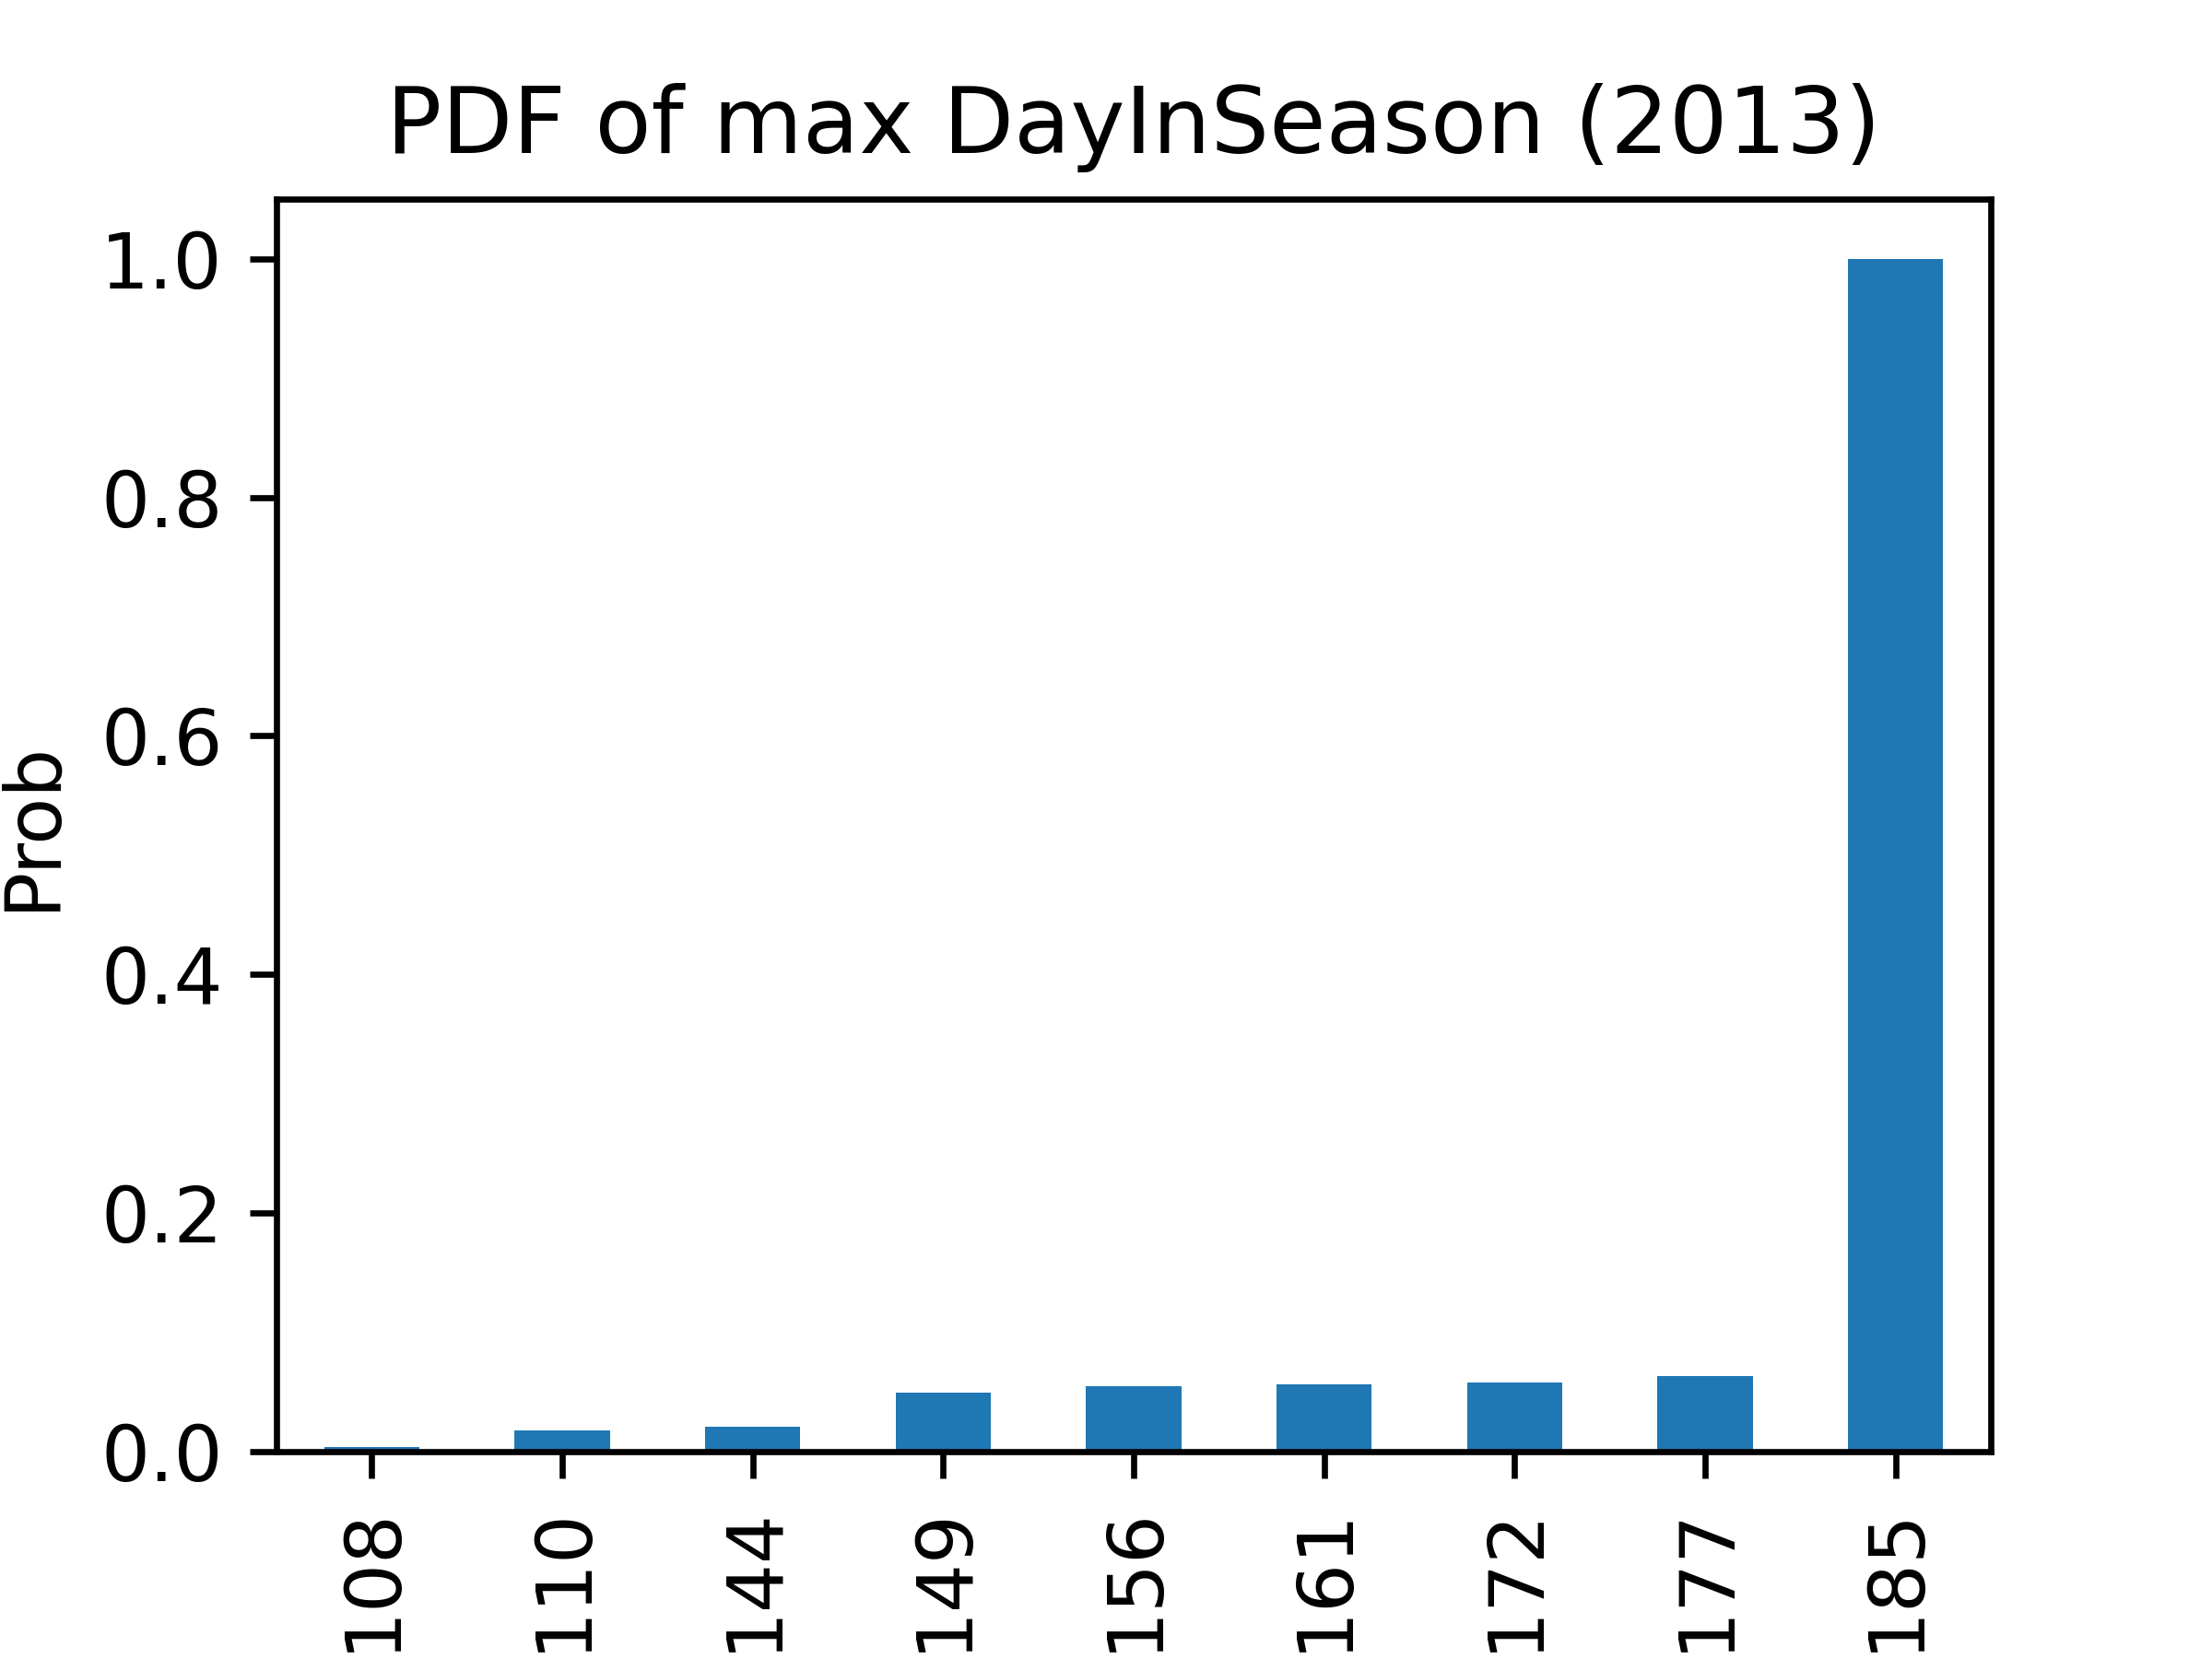
\includegraphics[width=0.45\linewidth]{./figures/PDF of max DayInSeason (2013).png}}
    \hfill
  \subfloat[\label{1b}]{%
        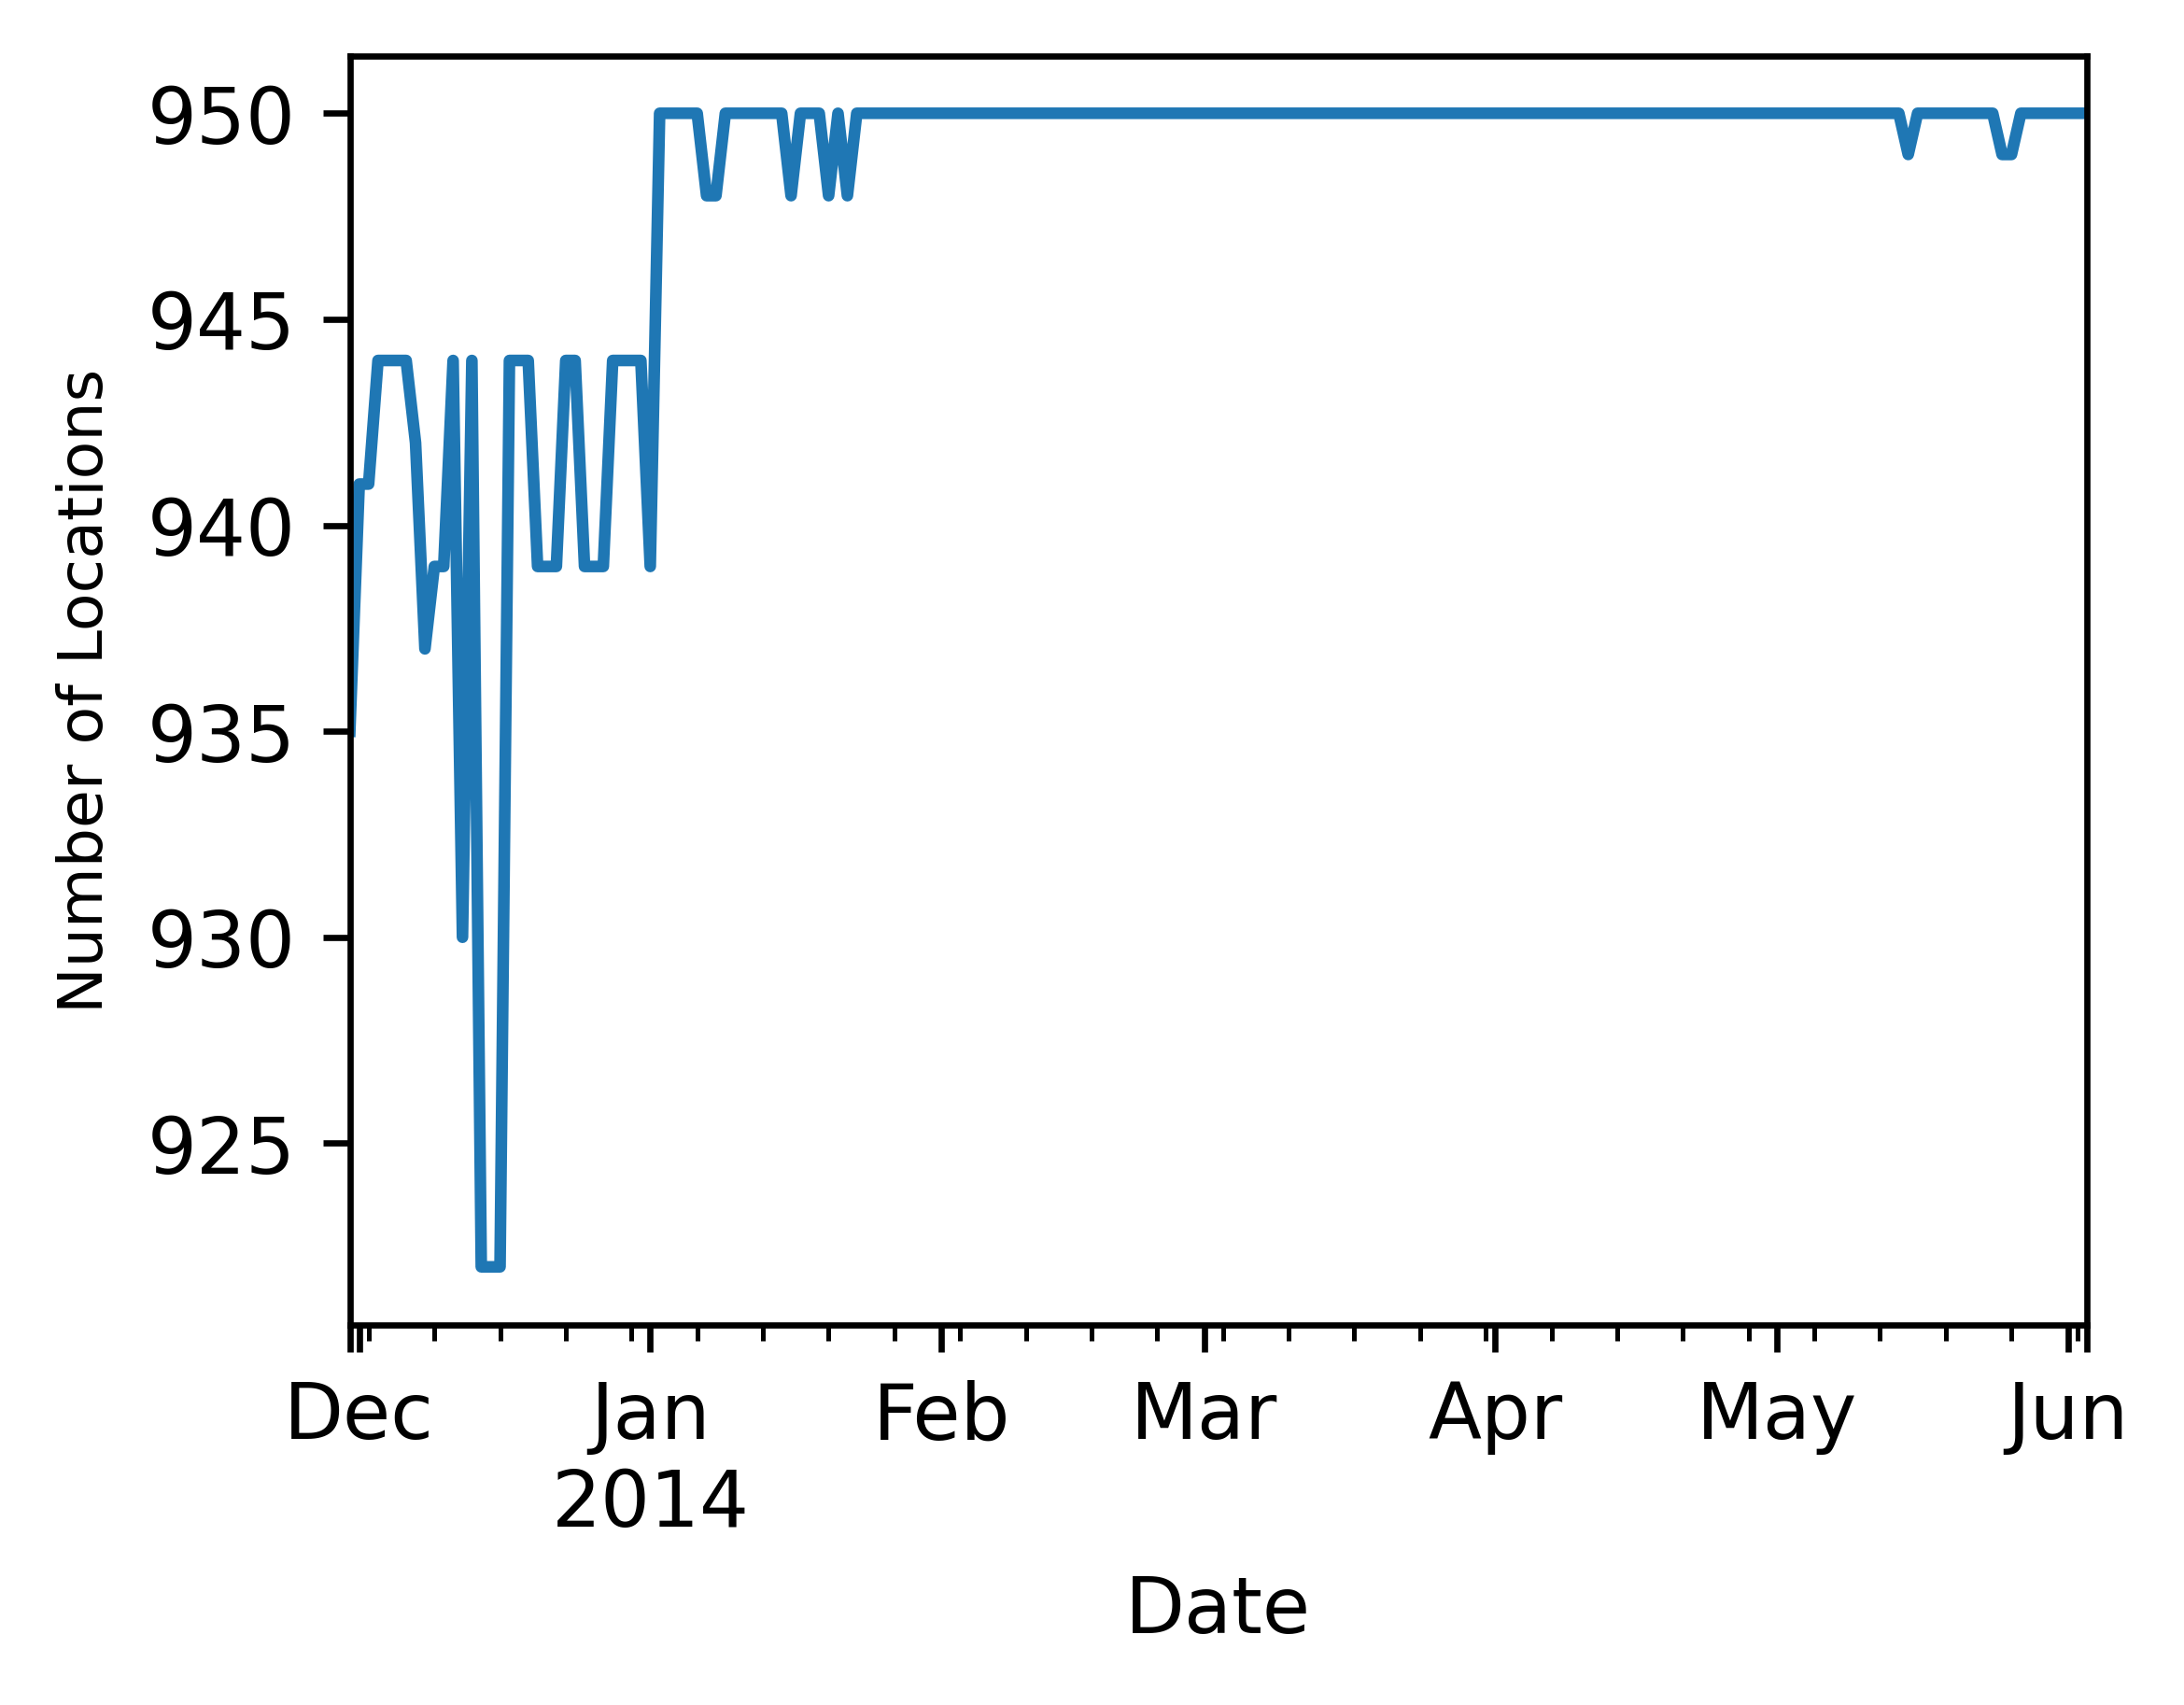
\includegraphics[width=0.45\linewidth]{./figures/date&locations(origin).png}}
    \\
  \subfloat[\label{1c}]{%
        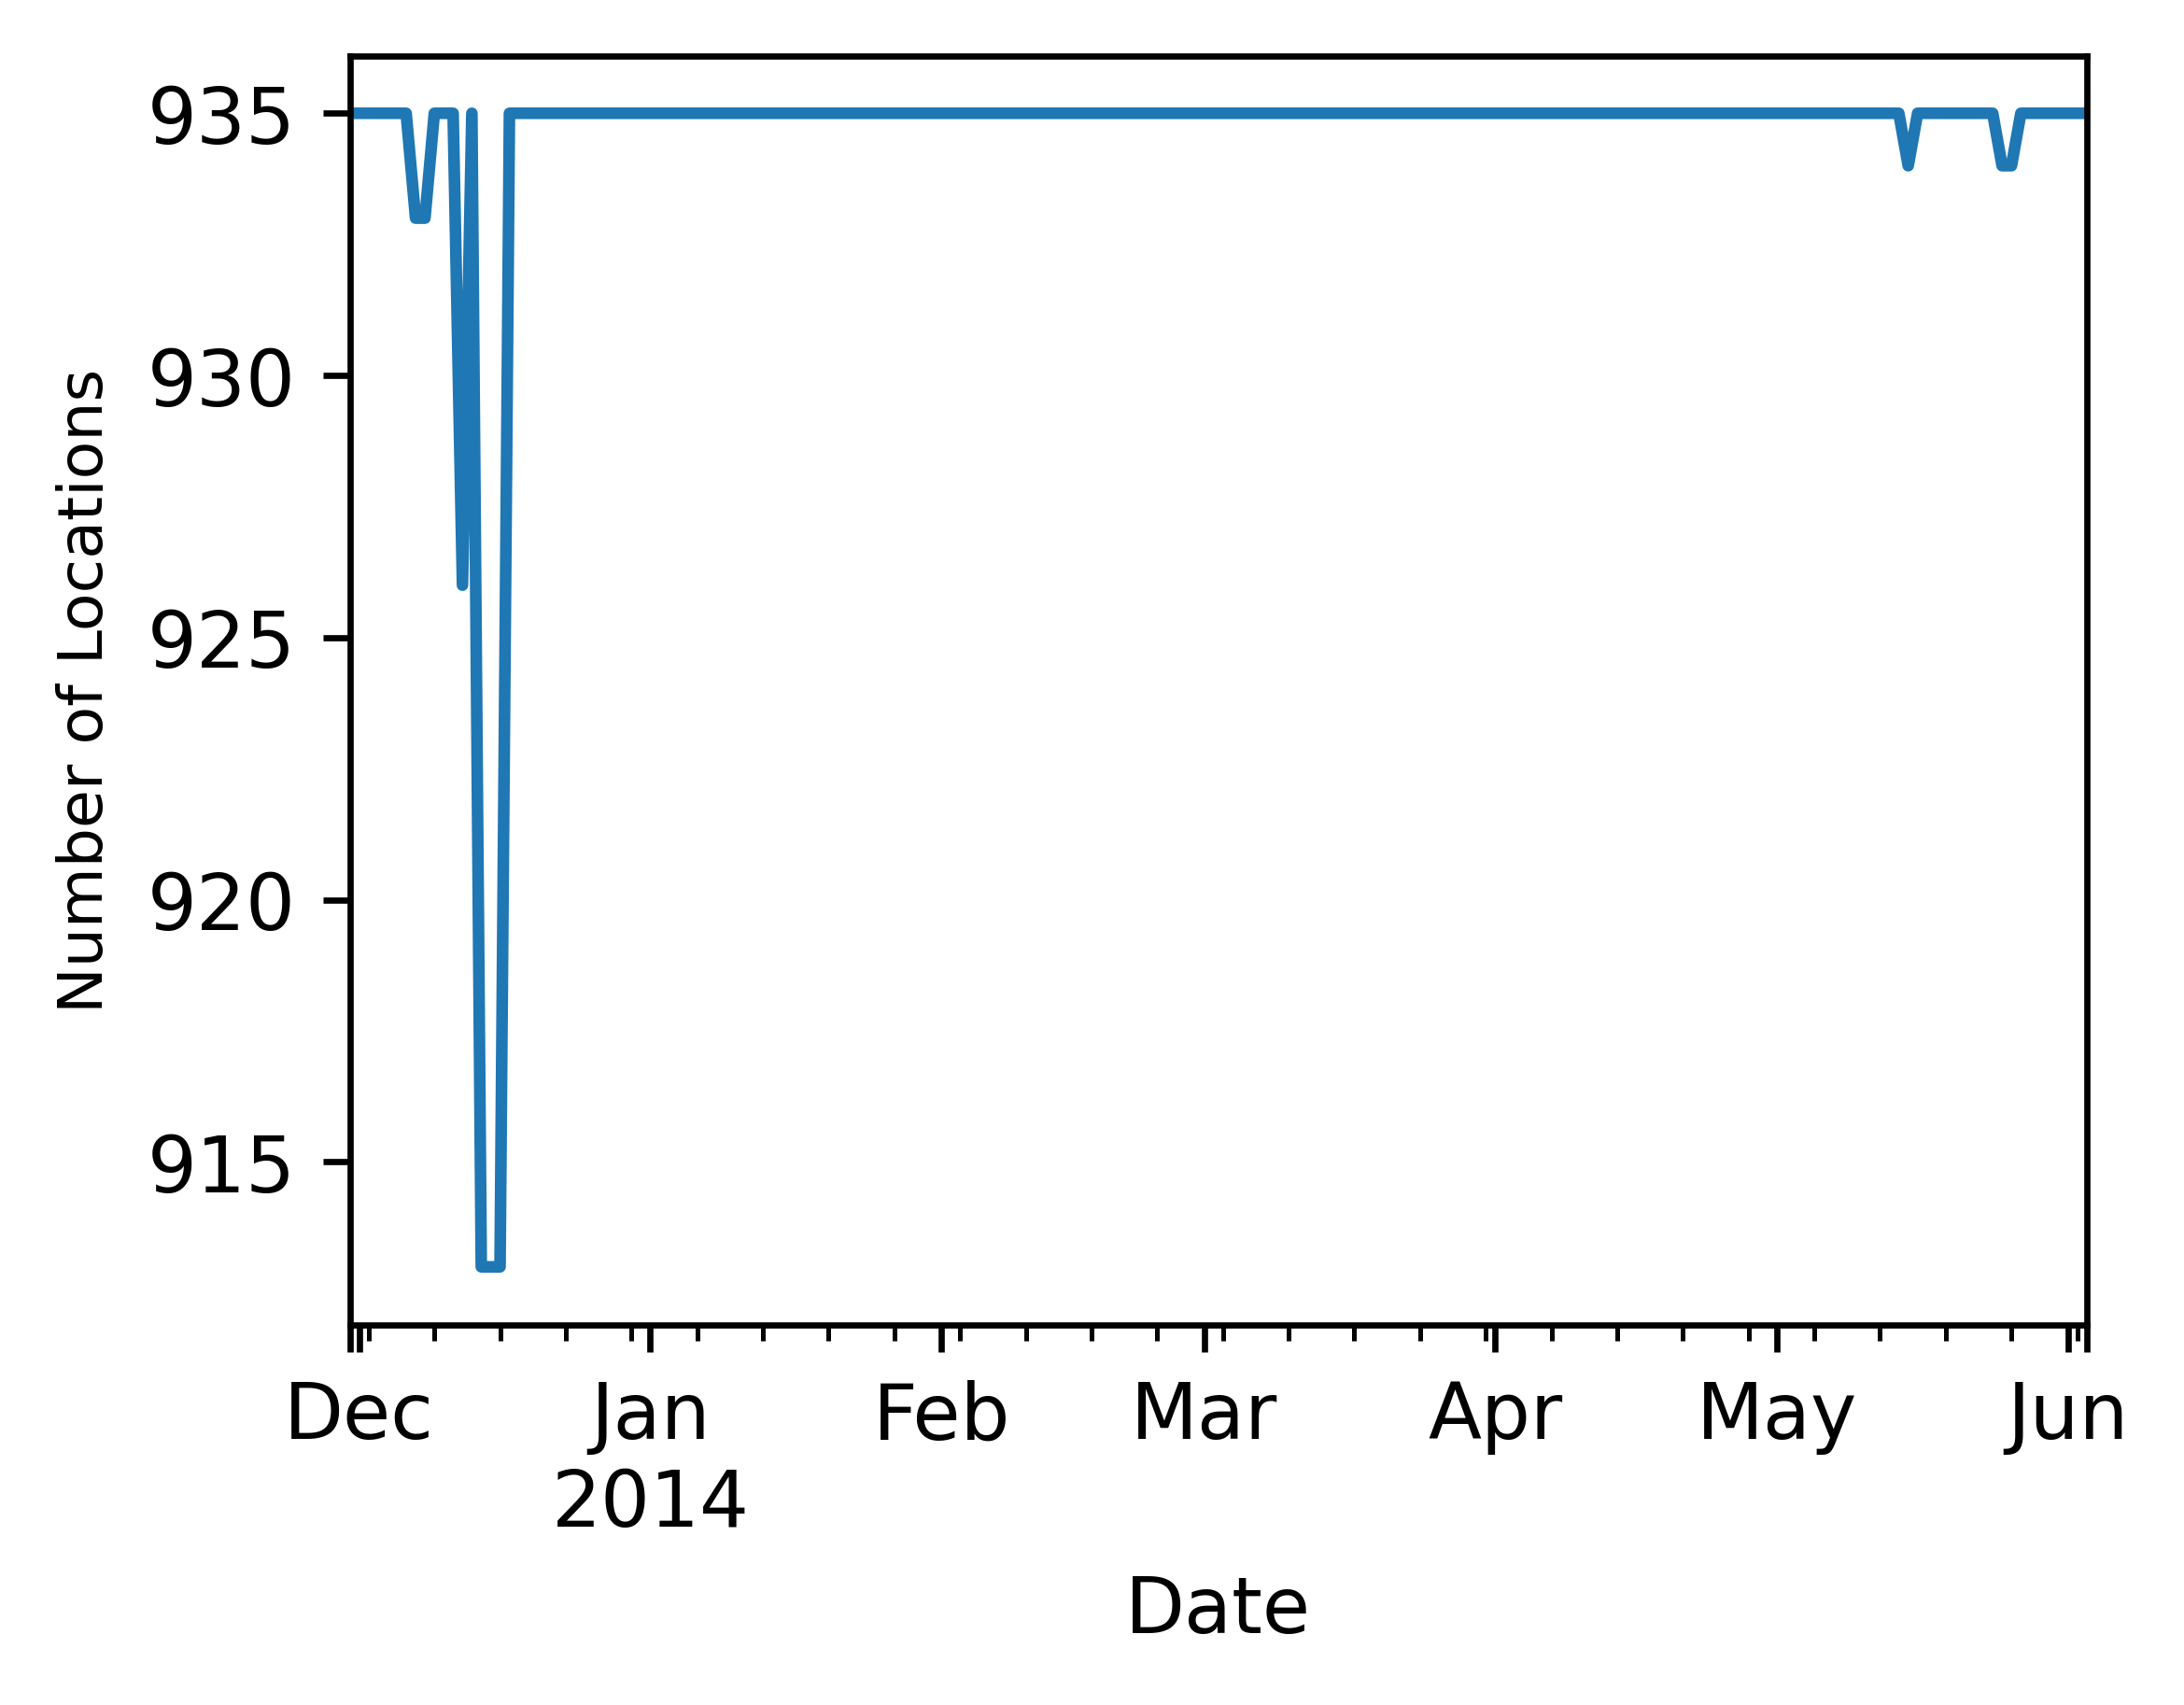
\includegraphics[width=0.45\linewidth]{./figures/date&locations.png}}
    \hfill
  \subfloat[\label{1d}]{%
        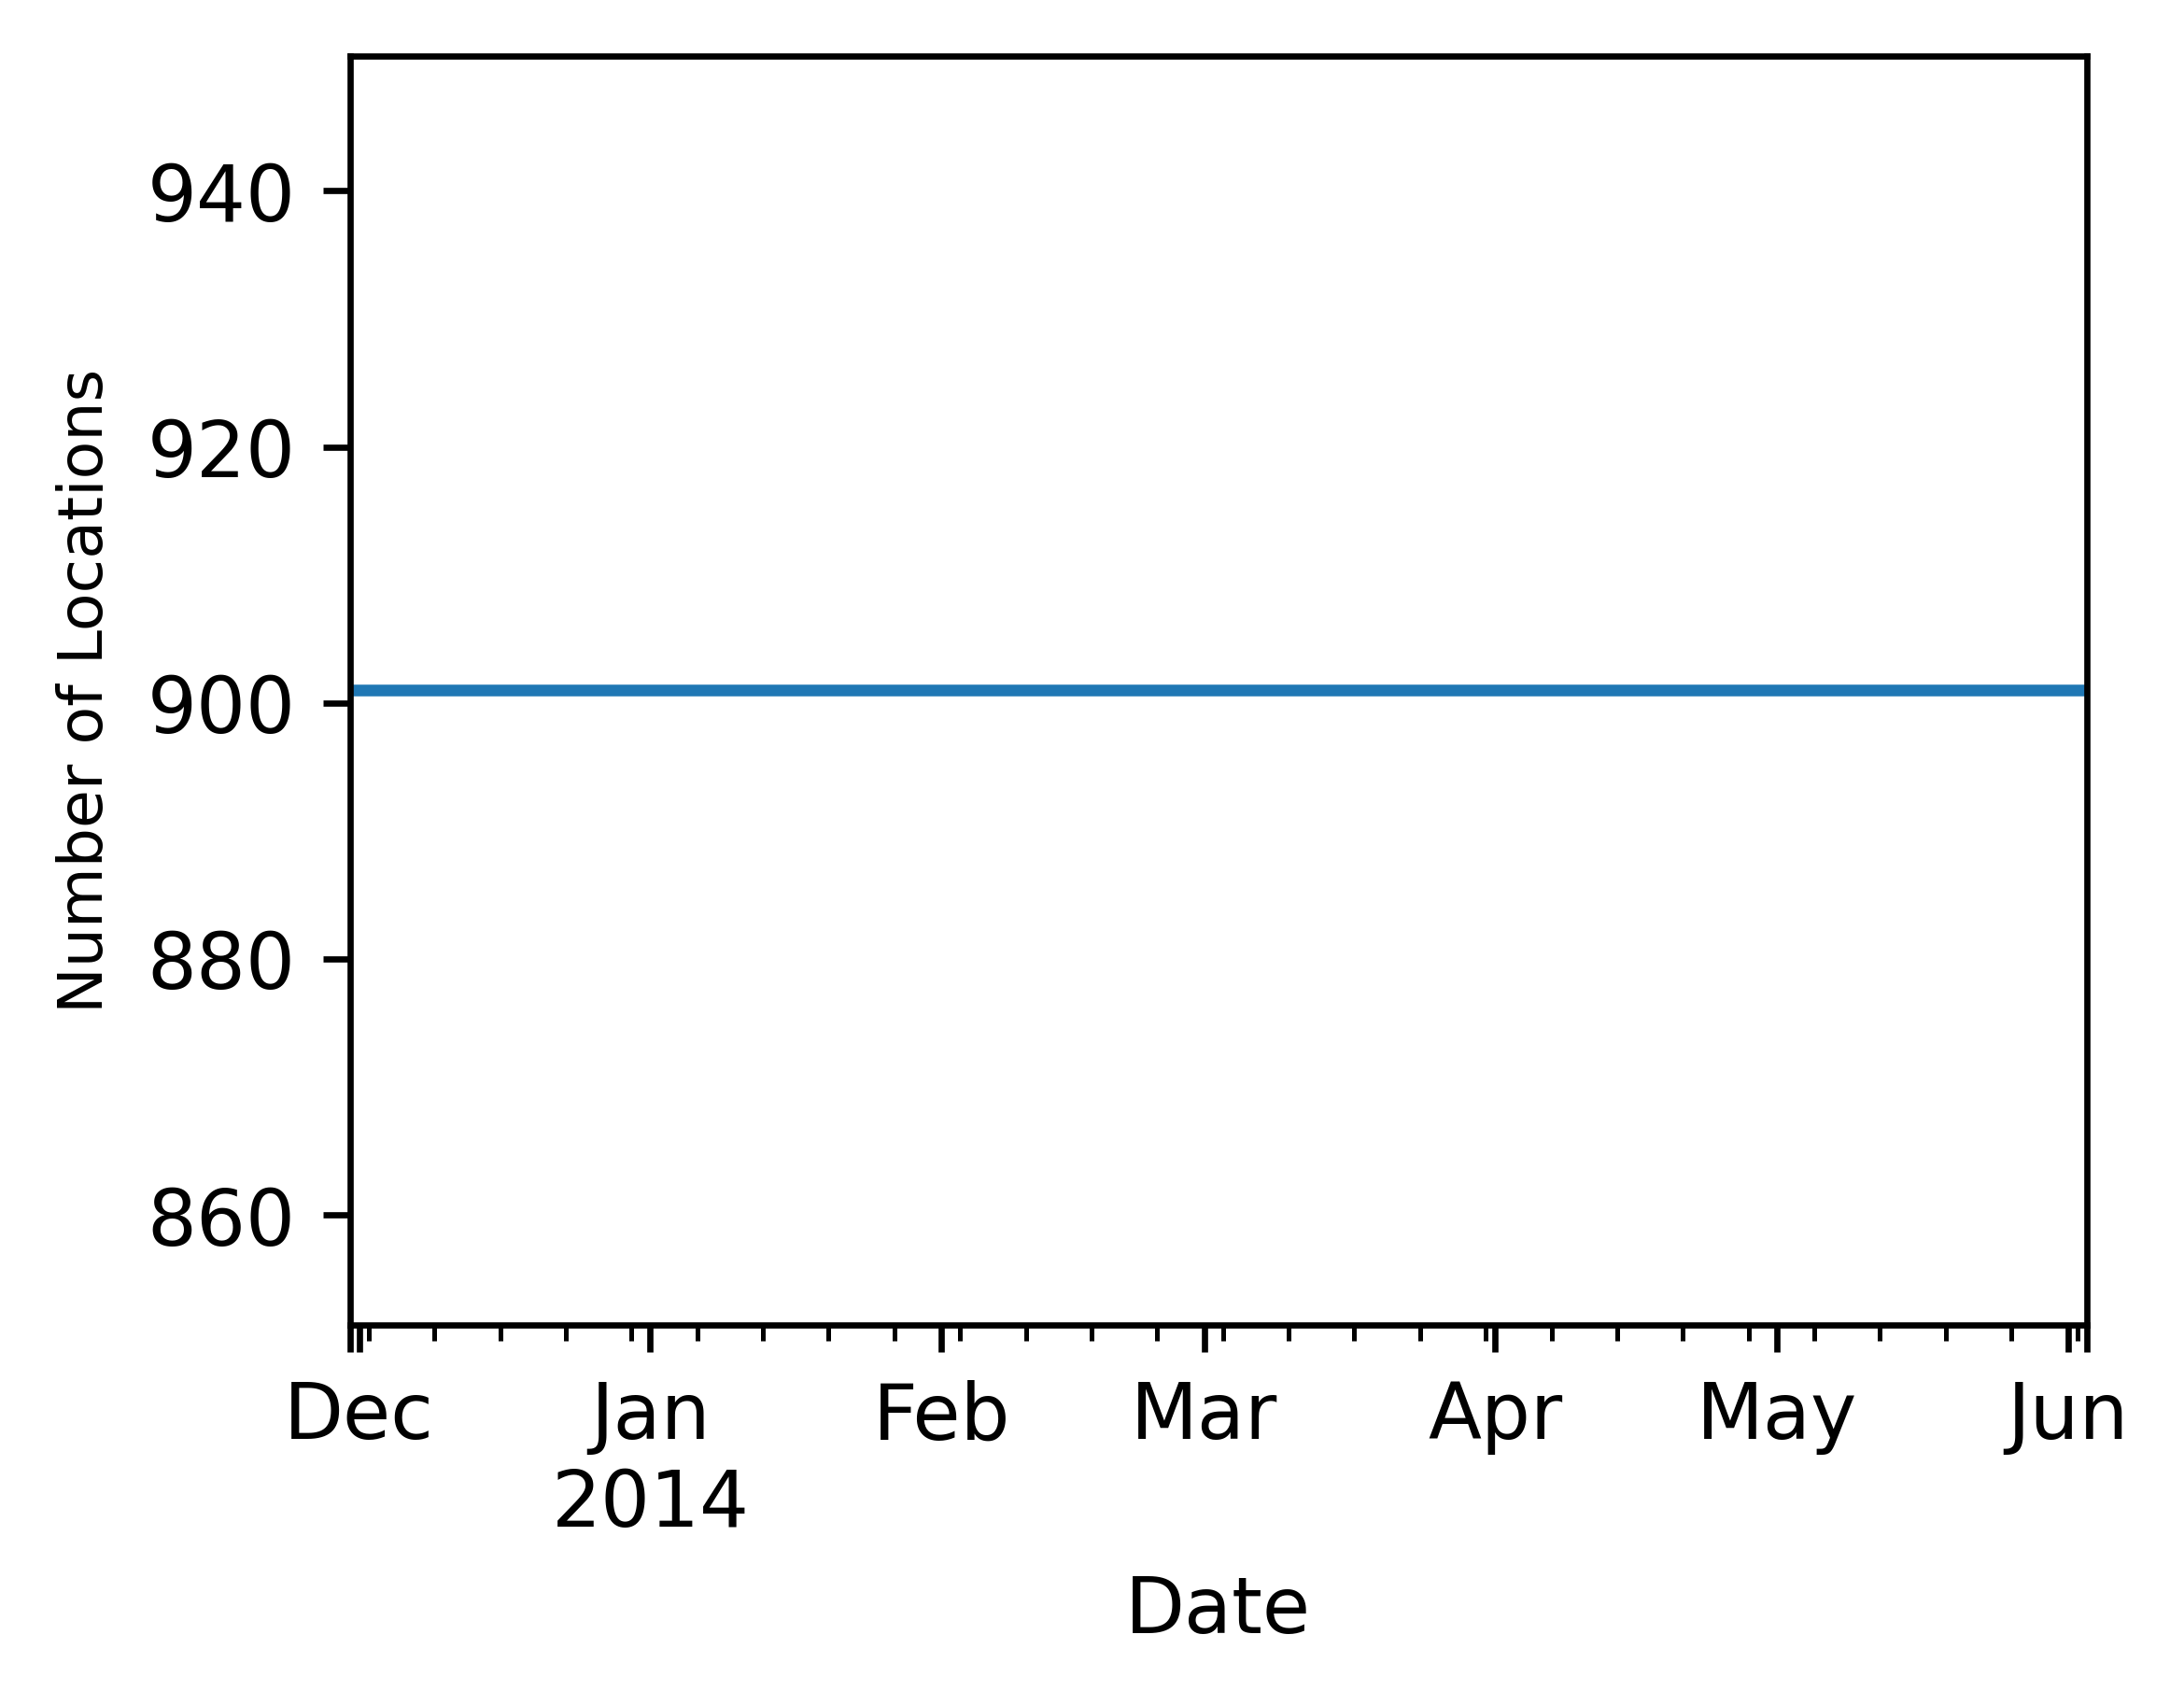
\includegraphics[width=0.45\linewidth]{./figures/date&locations(clean).png}}
  \caption{Missing data processing}
  \label{fig:missing-data} 
\end{figure}

\subsection{Map visualization}
  For data with location, map visualization can always help us find some intuitive relations between location and target. According to Fig.~\ref{fig:Map_visual}-(b), there are two intuitive conclusions:
\begin{itemize}
    \item The yield in the northern growing areas was significantly higher than that in the south. 
    \item In the south growing areas, the more east the locations are the high the yields.
\end{itemize}

\begin{figure*}[!htb]
    \centering
  \subfloat[\label{mapa}]{%
       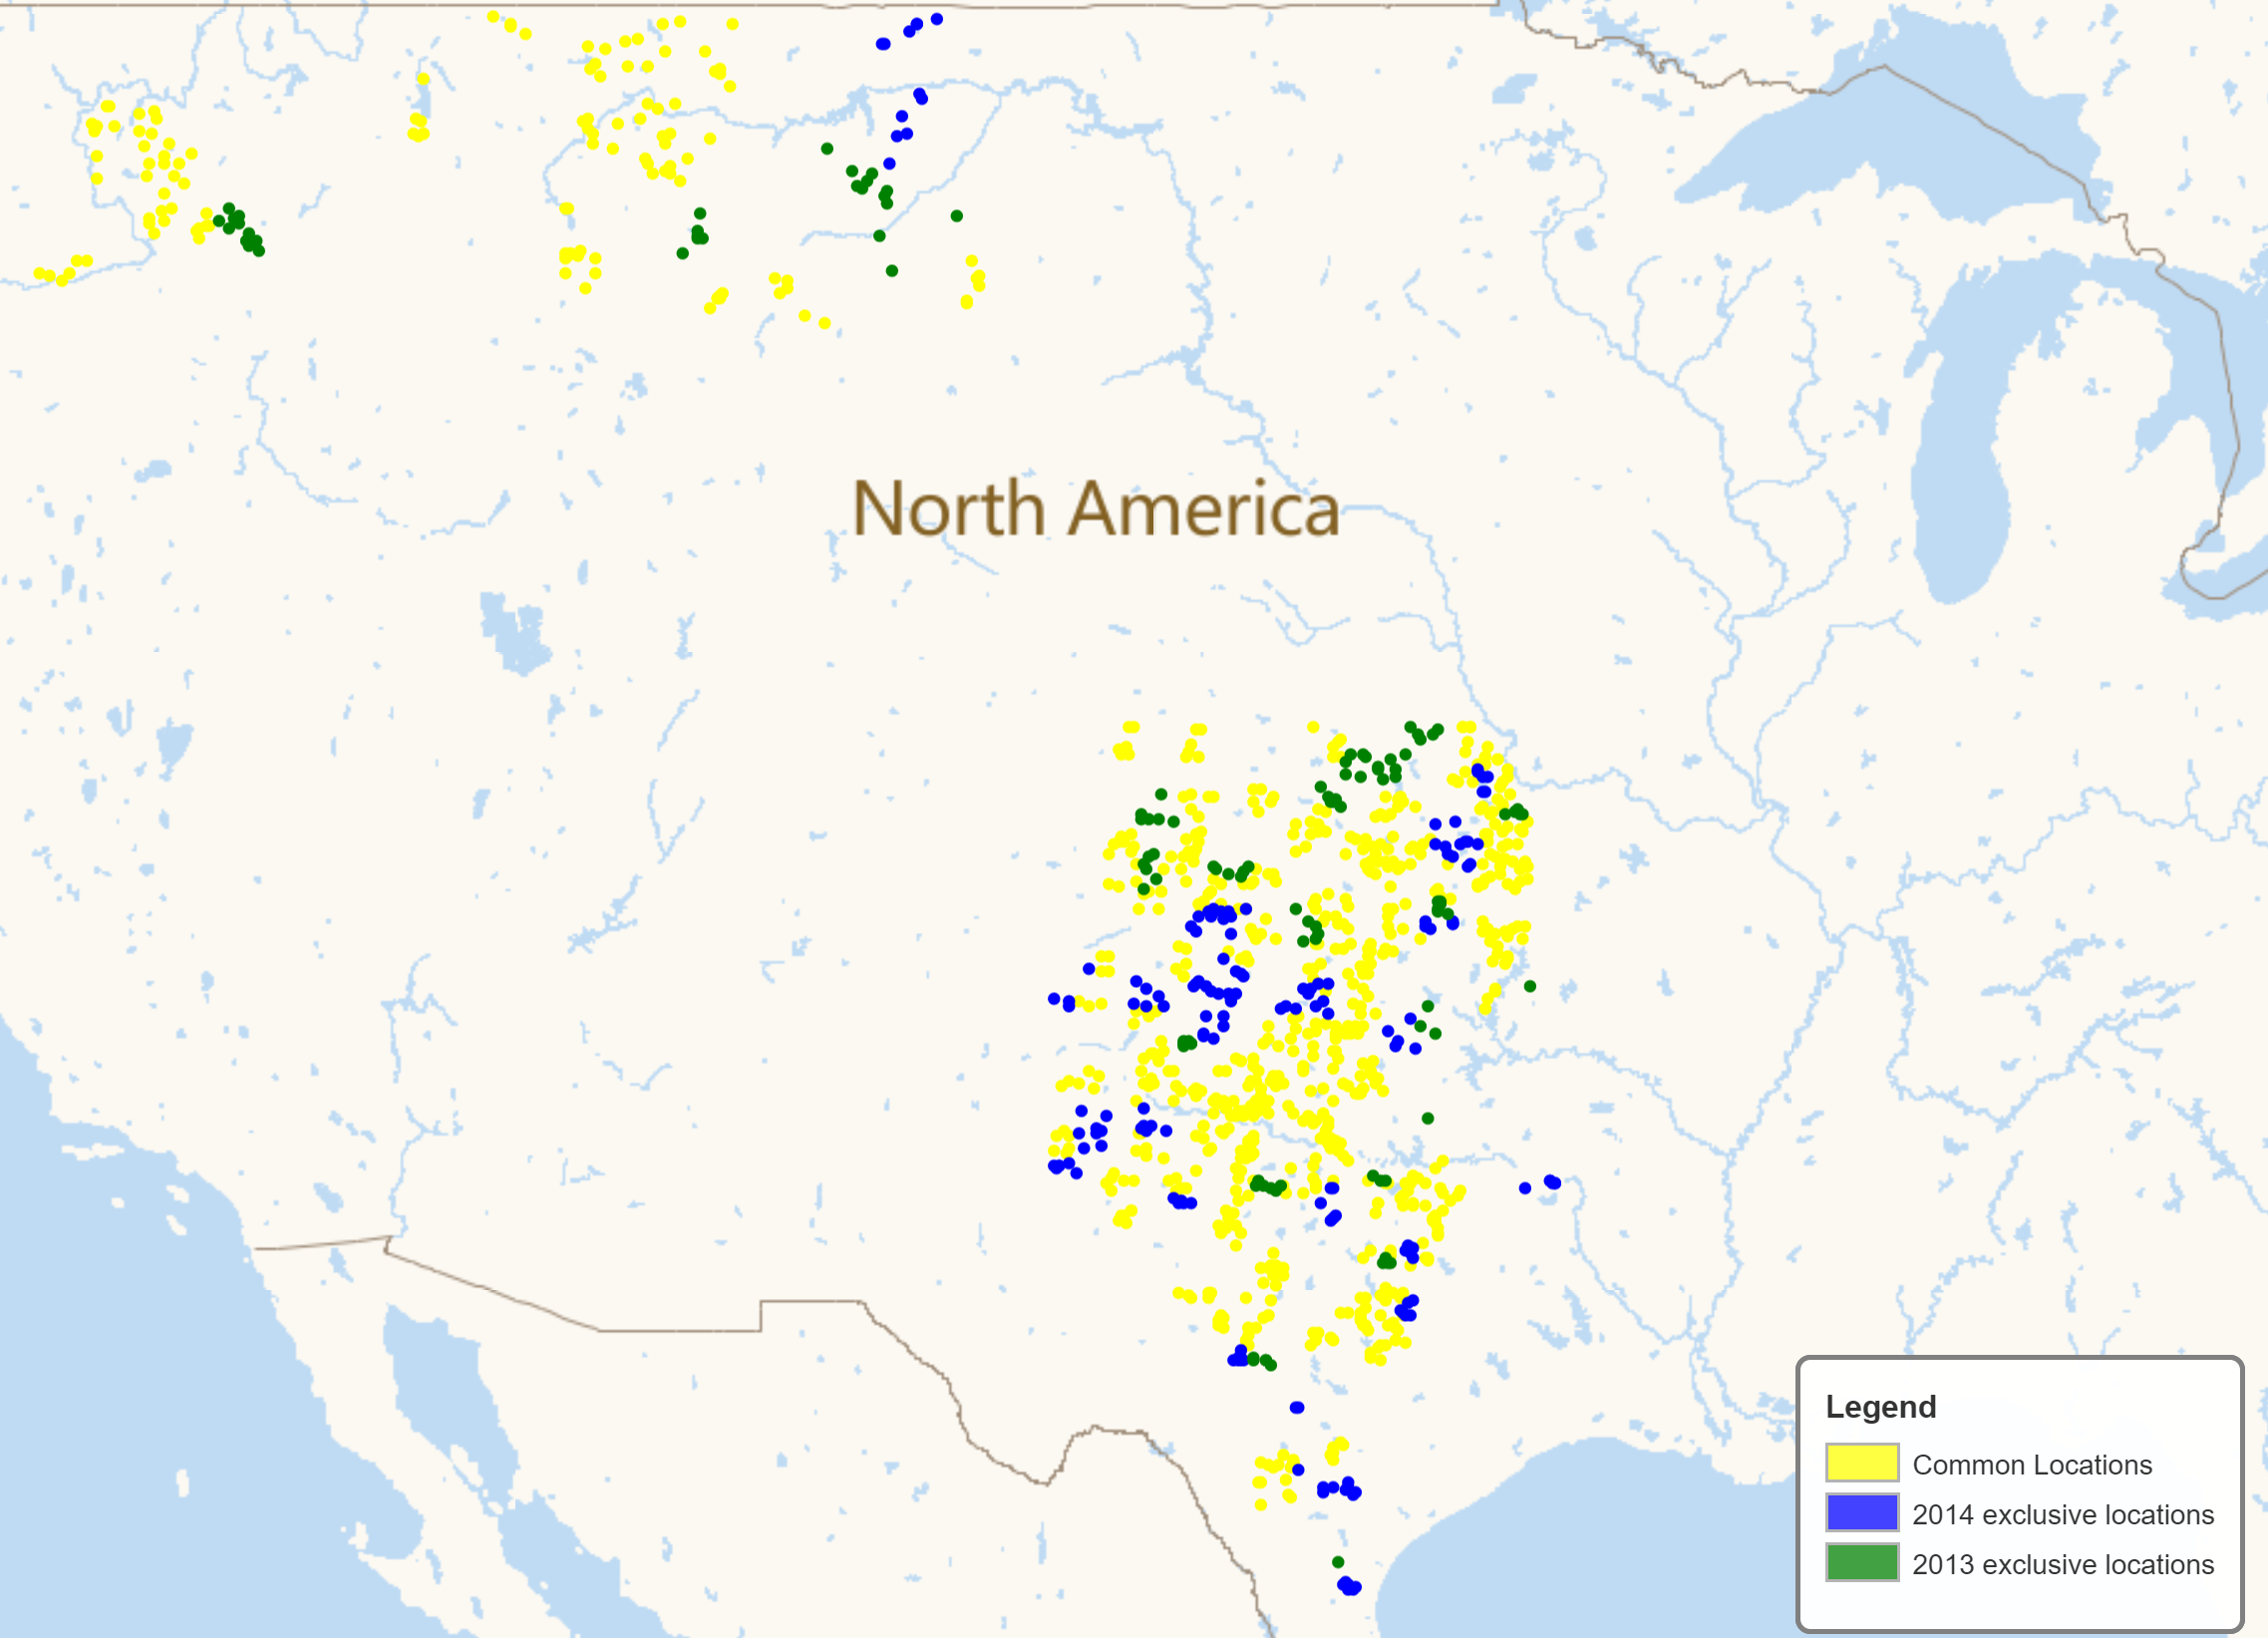
\includegraphics[width=0.45\linewidth]{./figures/data_locations.png}}
    \hfill
  \subfloat[\label{mapb}]{% TODO: replot figure 
        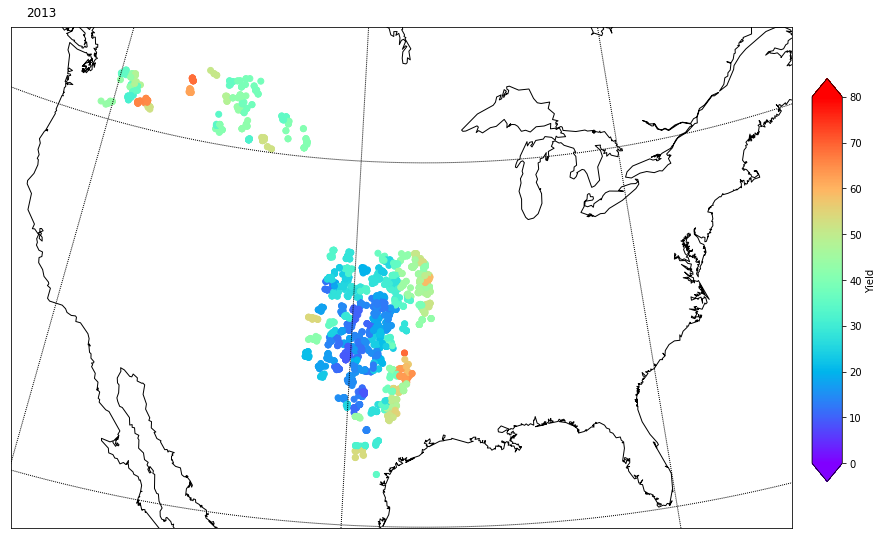
\includegraphics[width=0.45\linewidth]{./figures/yield&loc.png}}
  \label{fig:Map_visual} 
  \caption{(a)shows the location of all data being collected, yellow points represent locations monitered for two years which can be used for forecasting next year's yields via data of previous years. (b)shows the yeild varying by locations}
\end{figure*}

\subsection{Feature selection}
  There are significant multicollinearity between some features in the data, which can lead to errors and distortions in the results\cite{farrar1967multicollinearity}. By calculating the correlation coefficient between the features, findding that there are features with correlation higher than 90\% with another, some even reach 99\%. Table.~\ref{tab:correlation} shows the features correlation high than 90\%, these features accompanied with some other features unrelated to target such as \textit{State}, \textit{Date} e.t. 
\begin{table}[htbp]
\caption{Features correlation high than 90\%}
\begin{center}
\begin{tabular}{|c|c|c|c|c|}
\hline
Feature 1 & Feature 2 & cor1 & cor2 & cor3\\
\hline
apparentTempMin & TempMin     & 0.99 & -0.04 & -0.06 \\
apparentTempMax & TempMax     & 0.99 & -0.14 & -0.15 \\
precipIntensity & precipIntensityMax & 0.91 & 0.04  & 0.03  \\
dewPoint & tempMin & 0.91 & 0.01  & -0.06 \\
apparentTempMin & dewPoint & 0.90 & -0.04 & 0.01 \\
\hline
\multicolumn{5}{l}{$^{\mathrm{a}}$cor1: correlation between feature1 and feture2} \\
\multicolumn{5}{l}{$^{\mathrm{b}}$cor2: correlation between feature1 and yeild} \\ 
\multicolumn{5}{l}{$^{\mathrm{c}}$cor3: correlation between feature2 and yeild} \\
\end{tabular}
\label{tab:correlation}
\end{center}
\end{table}




\section{Bi-LSTM Model} \label{sec:model}
\subsection{LSTM}
  Recurrent Neural Network is a kind of neural network that is good at processing time series data. It can well process task with continuous time and contextual relationship wich is exactly in line with the characteristics of the crop growth. The connections existing between each layer make the network better in learing time series relations, but on the other hand, this leads to gradient explosion in backpropagation. \cite{hochreiter1997long}

\begin{figure}[htbp]
  \centerline{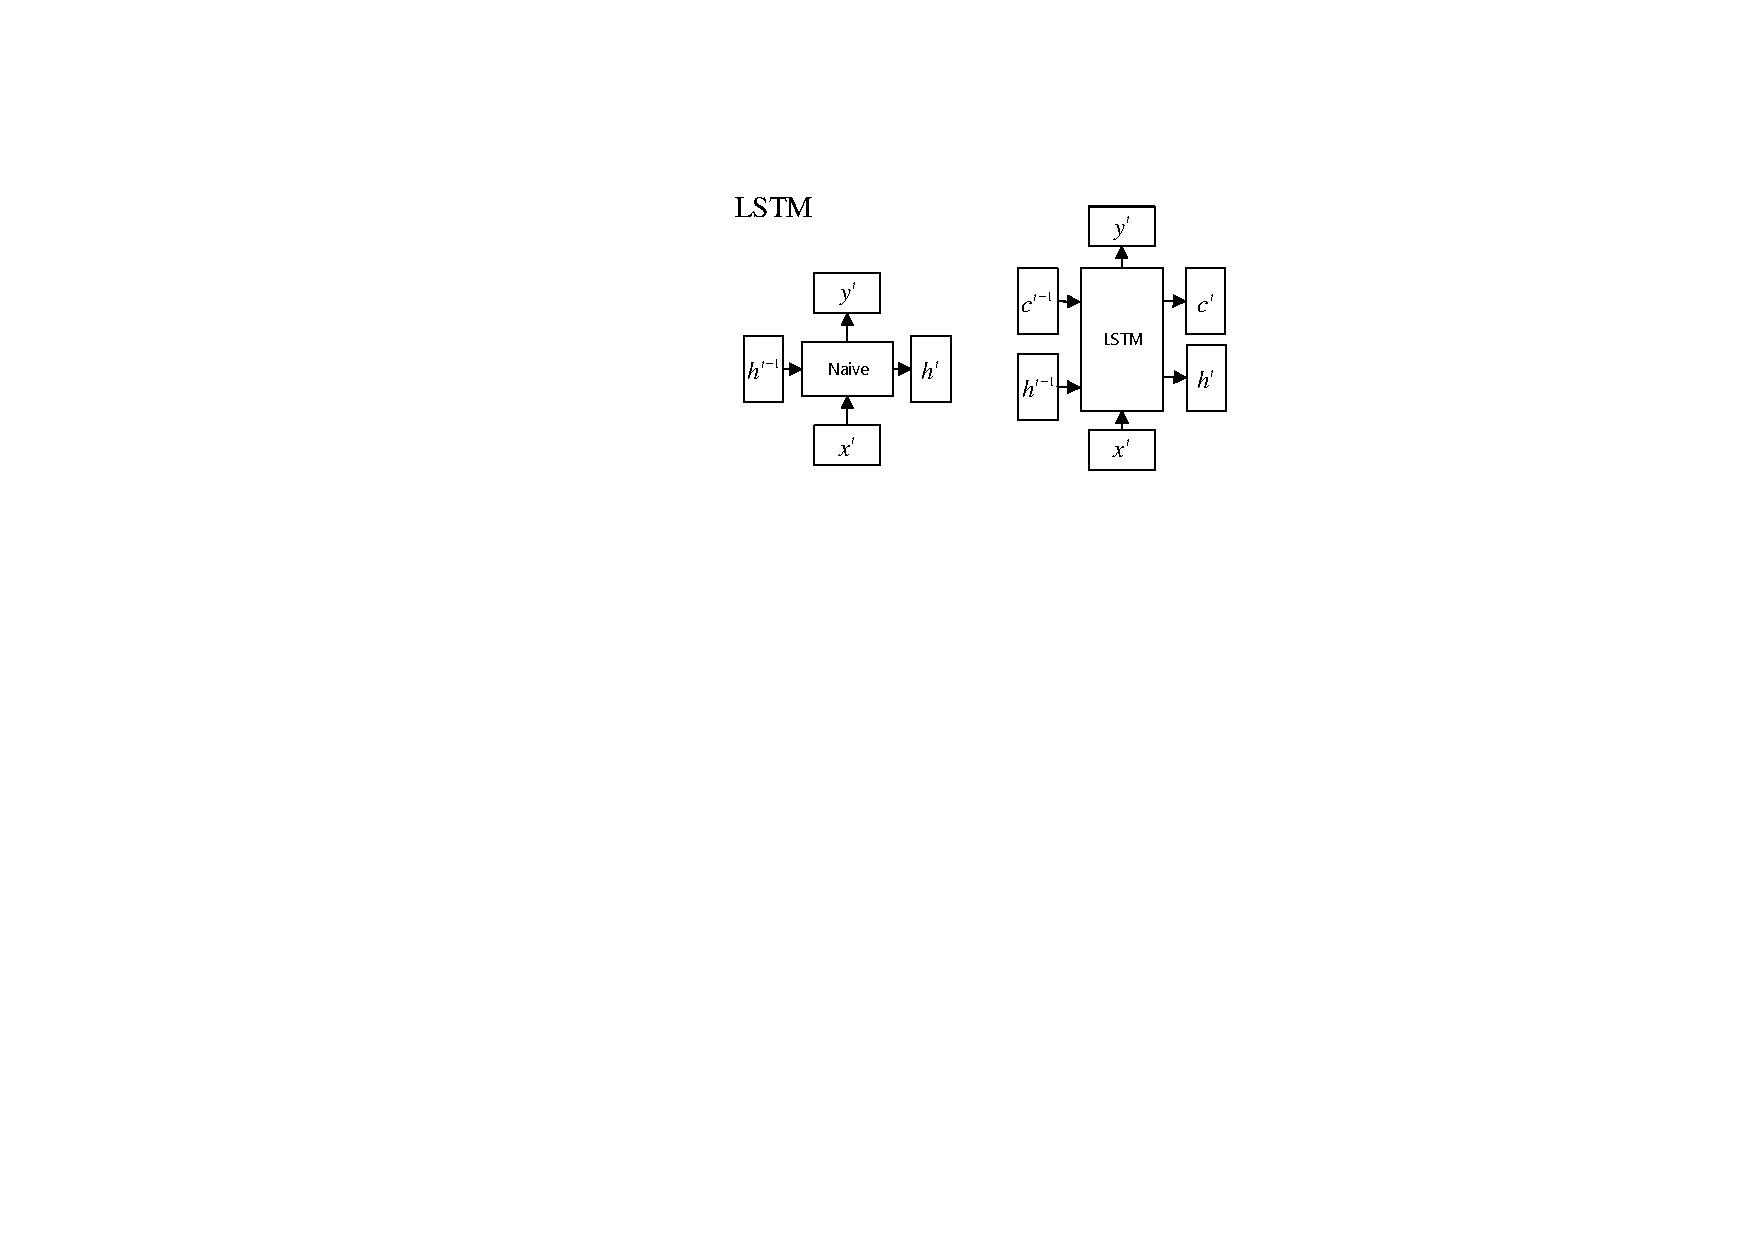
\includegraphics[width=0.7\linewidth]{figures/LSTM_struc.pdf}}
  \caption{LSTM and RNN structure}
  \label{fig:LSTM}
\end{figure}

  Fig.~\ref{fig:LSTM} shows the structure of LSTM and RNN. The structure of t-th RNN node is on the first image, $x^t$ is the input of t-th node, $h^{t-1}$ is the input of t-th node recived from $t-1$th node, $y^t$is the output and $h^t$ is the output which transfer to next node, while LSTM have two more states $c^t$(cell state) and $h^t$(hidden state), state $c$ in LSTM is the counterpart of state $h$ in RNN, and normaly, state $c$ changes slowly in front propagation which typicaly to add a number to $c^{t-1}$. On the contrary, $h^t$ changes drasticly.

\begin{figure}[htbp]
  \centerline{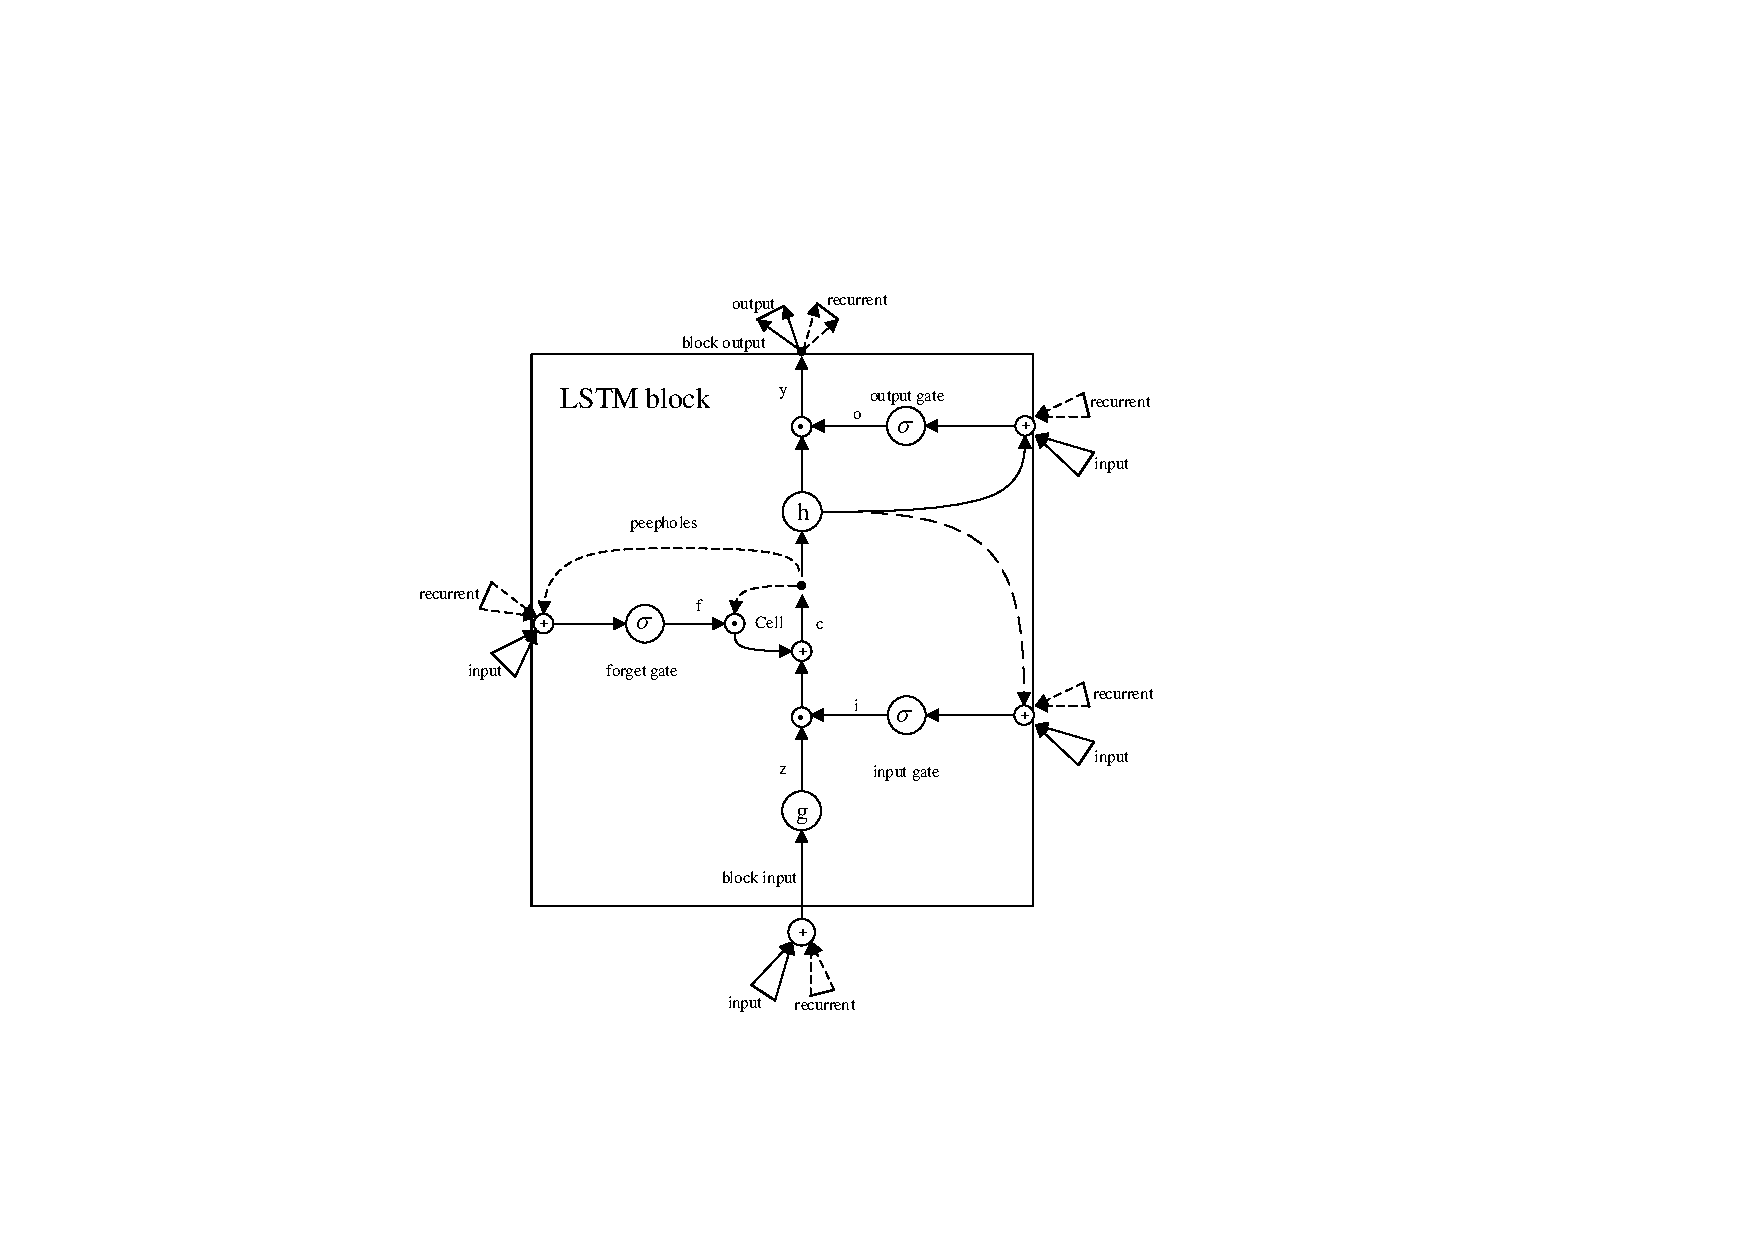
\includegraphics[width=0.7\linewidth]{figures/LSTM_node.pdf}}
  \caption{LSTM node}
  \label{fig:LSTM2}
\end{figure}

  For a LSTM node shown in Fig.~\ref{fig:LSTM2}, four states $f_t$(forget gate), $i_t$(input gate), $c_t$(current state) and $o_t$(output gate) are generated by concating $x^t$ and $h^{t-1}$ via (\ref{eq:gate}). Forget gate $f_t$ contral the remain of information transtered from $c_{t-1}$, $[h_{t-1}, x_t]$  means to concat vector $h_{t-1}$ and vector $x_t$, $w_f$ and $b_f$ are the weight and bias of forget gate $f_t$, $\sigma$ is the Sigmoid activate function, expression of Sigmoid is (\ref{eq:sigmoid}).

\begin{equation}
  \begin{cases}	f_t=\sigma \left( w_f\cdot \left[ h_{t-1},x_t \right] +b_f \right)\\	i_t=\sigma \left( w_i\cdot \left[ h_{t-1},x_t \right] +b_i \right)\\	o_t=\sigma \left( w_o\cdot \left[ h_{t-1},x_t \right] +b_i \right)\\\end{cases}
  \label{eq:gate}
\end{equation}

\begin{equation}
  \sigma \left( x \right) =\frac{1}{1+e^{-x}}
  \label{eq:sigmoid}
\end{equation}

To calculate $c_t$, the input state $\widetilde{c_t}$ are needed to be calculate first. Use activate function $\tanh$ via (\ref{eq:ct1}), (\ref{eq:ct2}) and (\ref{eq:gate}) to calculate $c_t$, the $\odot$ in (\ref{eq:ct2}) means corresponding element multiplication.

\begin{equation}
  \tilde{c}_t=\tanh \left( W_c\cdot \left[ h_{t-q},x_t \right] +b_c \right)
  \label{eq:ct1}
\end{equation}

\begin{equation}
  c_t=f_t\odot c_{t-1}+i_t\odot c_t
  \label{eq:ct2}
\end{equation}

All these features of LSTM meet the corp growing process, there are weather fluctuatuons or natural disasters in short time, while there are stable natural cinditions over a long period of time.

\subsection{Bi-LSTM Model}
As shown in Fig.~\ref{fig:model}, build Bi-LSTM network using Keras and Tensorflow, there are two parts in model. The left part is three layers of stacked Bi-LSTM use to predict the yield by the weather data, right part use stacked fully connected network to link the county and the predicted yield.



\begin{figure}[htbp]
  \centerline{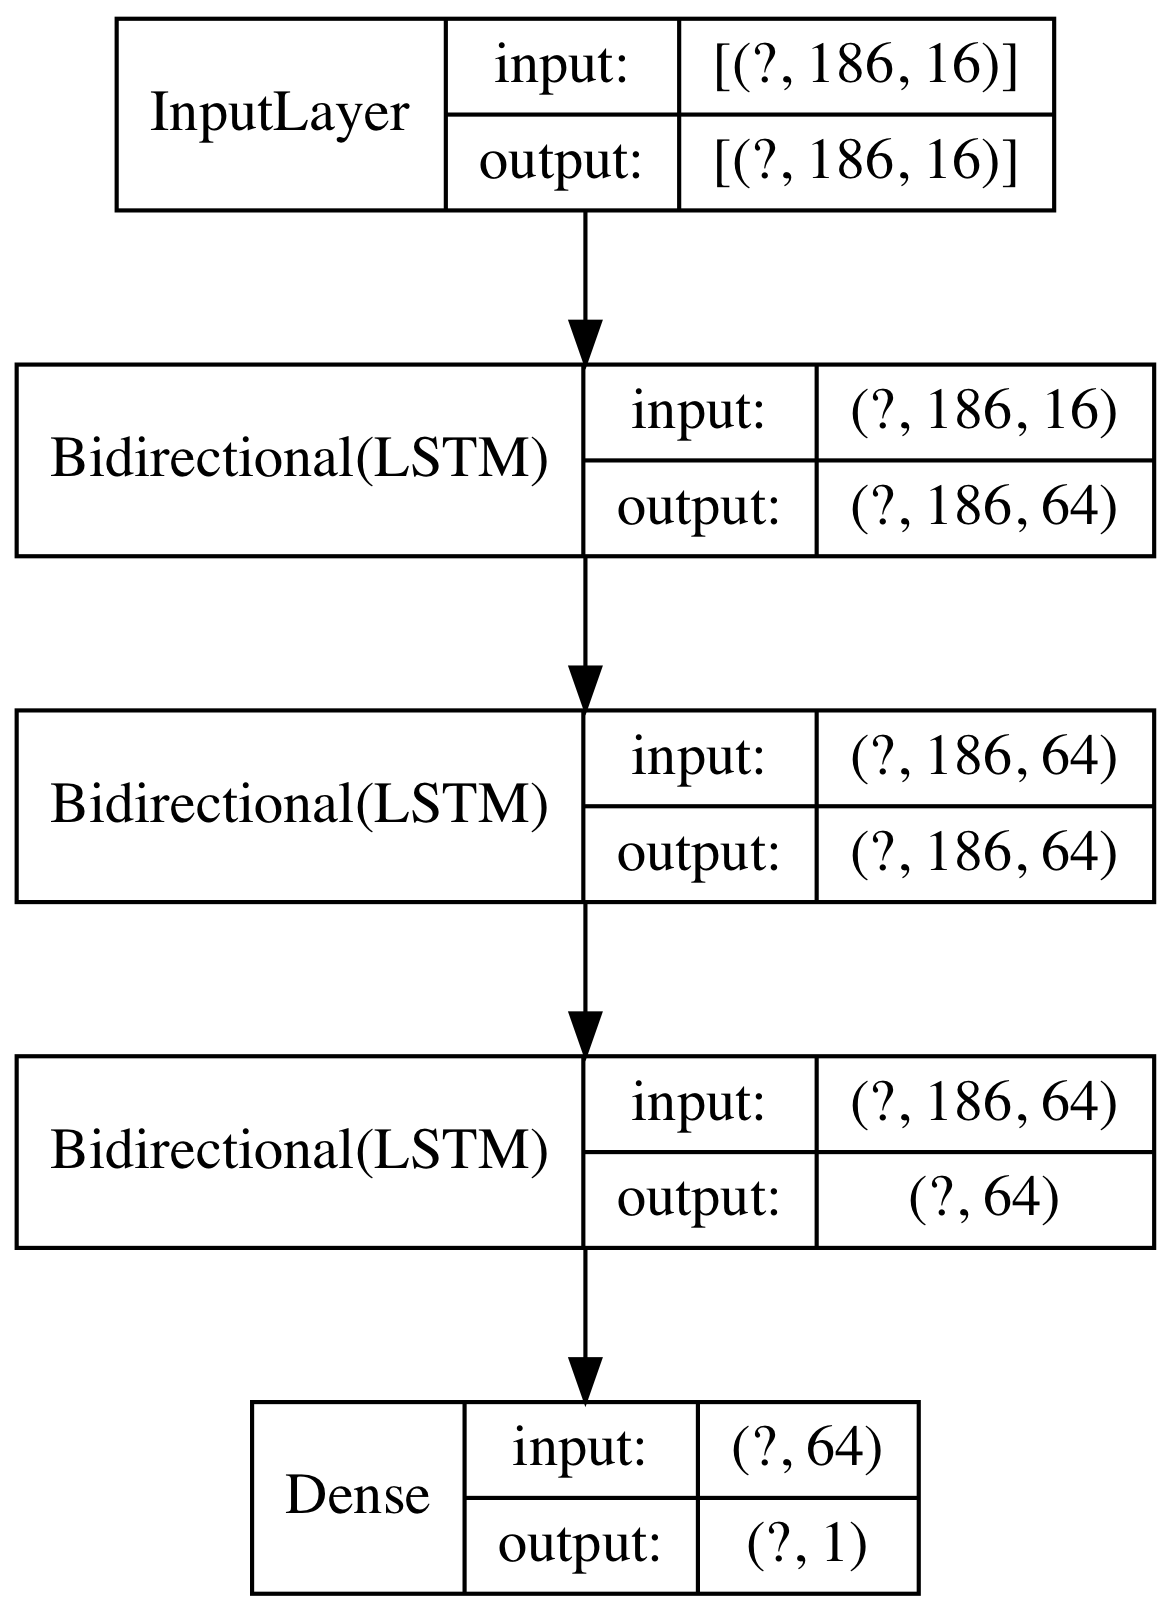
\includegraphics[width=\linewidth]{figures/Model_figure.png}}
  \caption{Bi-LSTM Model}
  \label{fig:model}
\end{figure}

\section{Experiment} \label{sec:ex}
\subsection{Test method}
Before testing, use \textit{Min-Max} method shown by (\ref{eq:standarlize}) to standarlize data and shuffle data due to the data is arranged by location. If not doing so, there will be data from new locations in train data while spliting the test set and train set.

\begin{equation}
  \frac{x_i-\min \left( x_i \right)}{\max \left( x_i \right) -\min \left( x_i \right)}
\label{eq:standarlize}
\end{equation}

Because the time complexity of SVR is more than twice of the data size\cite{clarke2005analysis}, extract 10000 entries of data in order to reduce time, randomly extract and run multiple times to avoid accidental exceptions caused by extraction.



\subsection{Test Result}
The result of algorithm test is as shown in Table.~\ref{tab:result}, and RF shows a severe overfiting among all the algoritms. The prediction contribution of features shown in Table.~\ref{tab:RF_contribution}, it is obviously that yield prediction is dominated by loction.

\begin{table}[htbp]
  \caption{Performance of algrorithms on corp yield prediction}
  \begin{center}
  \begin{tabular}{|c|c|}
  \hline
  Algorithm                                    & MSE      \\
  \hline
  Random Forest                                & 0.0048   \\
  Random Forest(10K)                           & 0.1096   \\
  KNN                                          & 60.6555  \\
  Polynomial regression                        & 108.4011 \\
  Polynomial regression with L2 regularization & 108.4891 \\
  Linear regression                            & 179.4249 \\
  Linear regression with L2 regularization     & 179.4339 \\
  SVR(1K)                                      & 188.4630 \\
  SVR RBF kernel(10K)                          & 193.5149 \\
  SVR linear kernel(10K)                       & 197.0644 \\
  Gradient boost                               & 231.4852 \\
  KRR                                          & 333.6586 \\
  \hline
  \multicolumn{2}{l}{$^{\mathrm{a}}$ 10K: Extract 10K entries of data to reduce training time} \\
  \end{tabular}
  \label{tab:result}
  \end{center}
\end{table}

\begin{table}[htbp]
    \caption{Feature contribution fo RF}
    \begin{center}
    \begin{tabular}{|c|c|}
    \hline
      Feature & Contribution \\
    \hline
      Longitude & 0.7656 \\
      Latitude & 0.2342 \\
      cloudCover & 0.0001 \\
    \hline
    \end{tabular}
    \label{tab:RF_contribution}
    \end{center}
\end{table}

Group the data by location and check the yield finding that the number of unique yields not match that of locations, which means there are entries share the same yield. Look further into data, finding that the yield of a day is not the real yield of current day, but the yield of final yield. What's more, the locations from the same conunty also share the same yield. That derectly results in loctions' neighborhoods get same yields, and the algorithm can give the exact yield according to the yield. 

\subsection{Overfitting in Random Forest}
Simply remove longitude and latitude form data and run test again, get the learning curve shown by Fig.~\ref{cv1}. Clearly, it is not the "location" leads to the overfitting, but the structure of data.

\begin{figure}[!htb]
  \centering
\subfloat[\label{cv1}]{%
     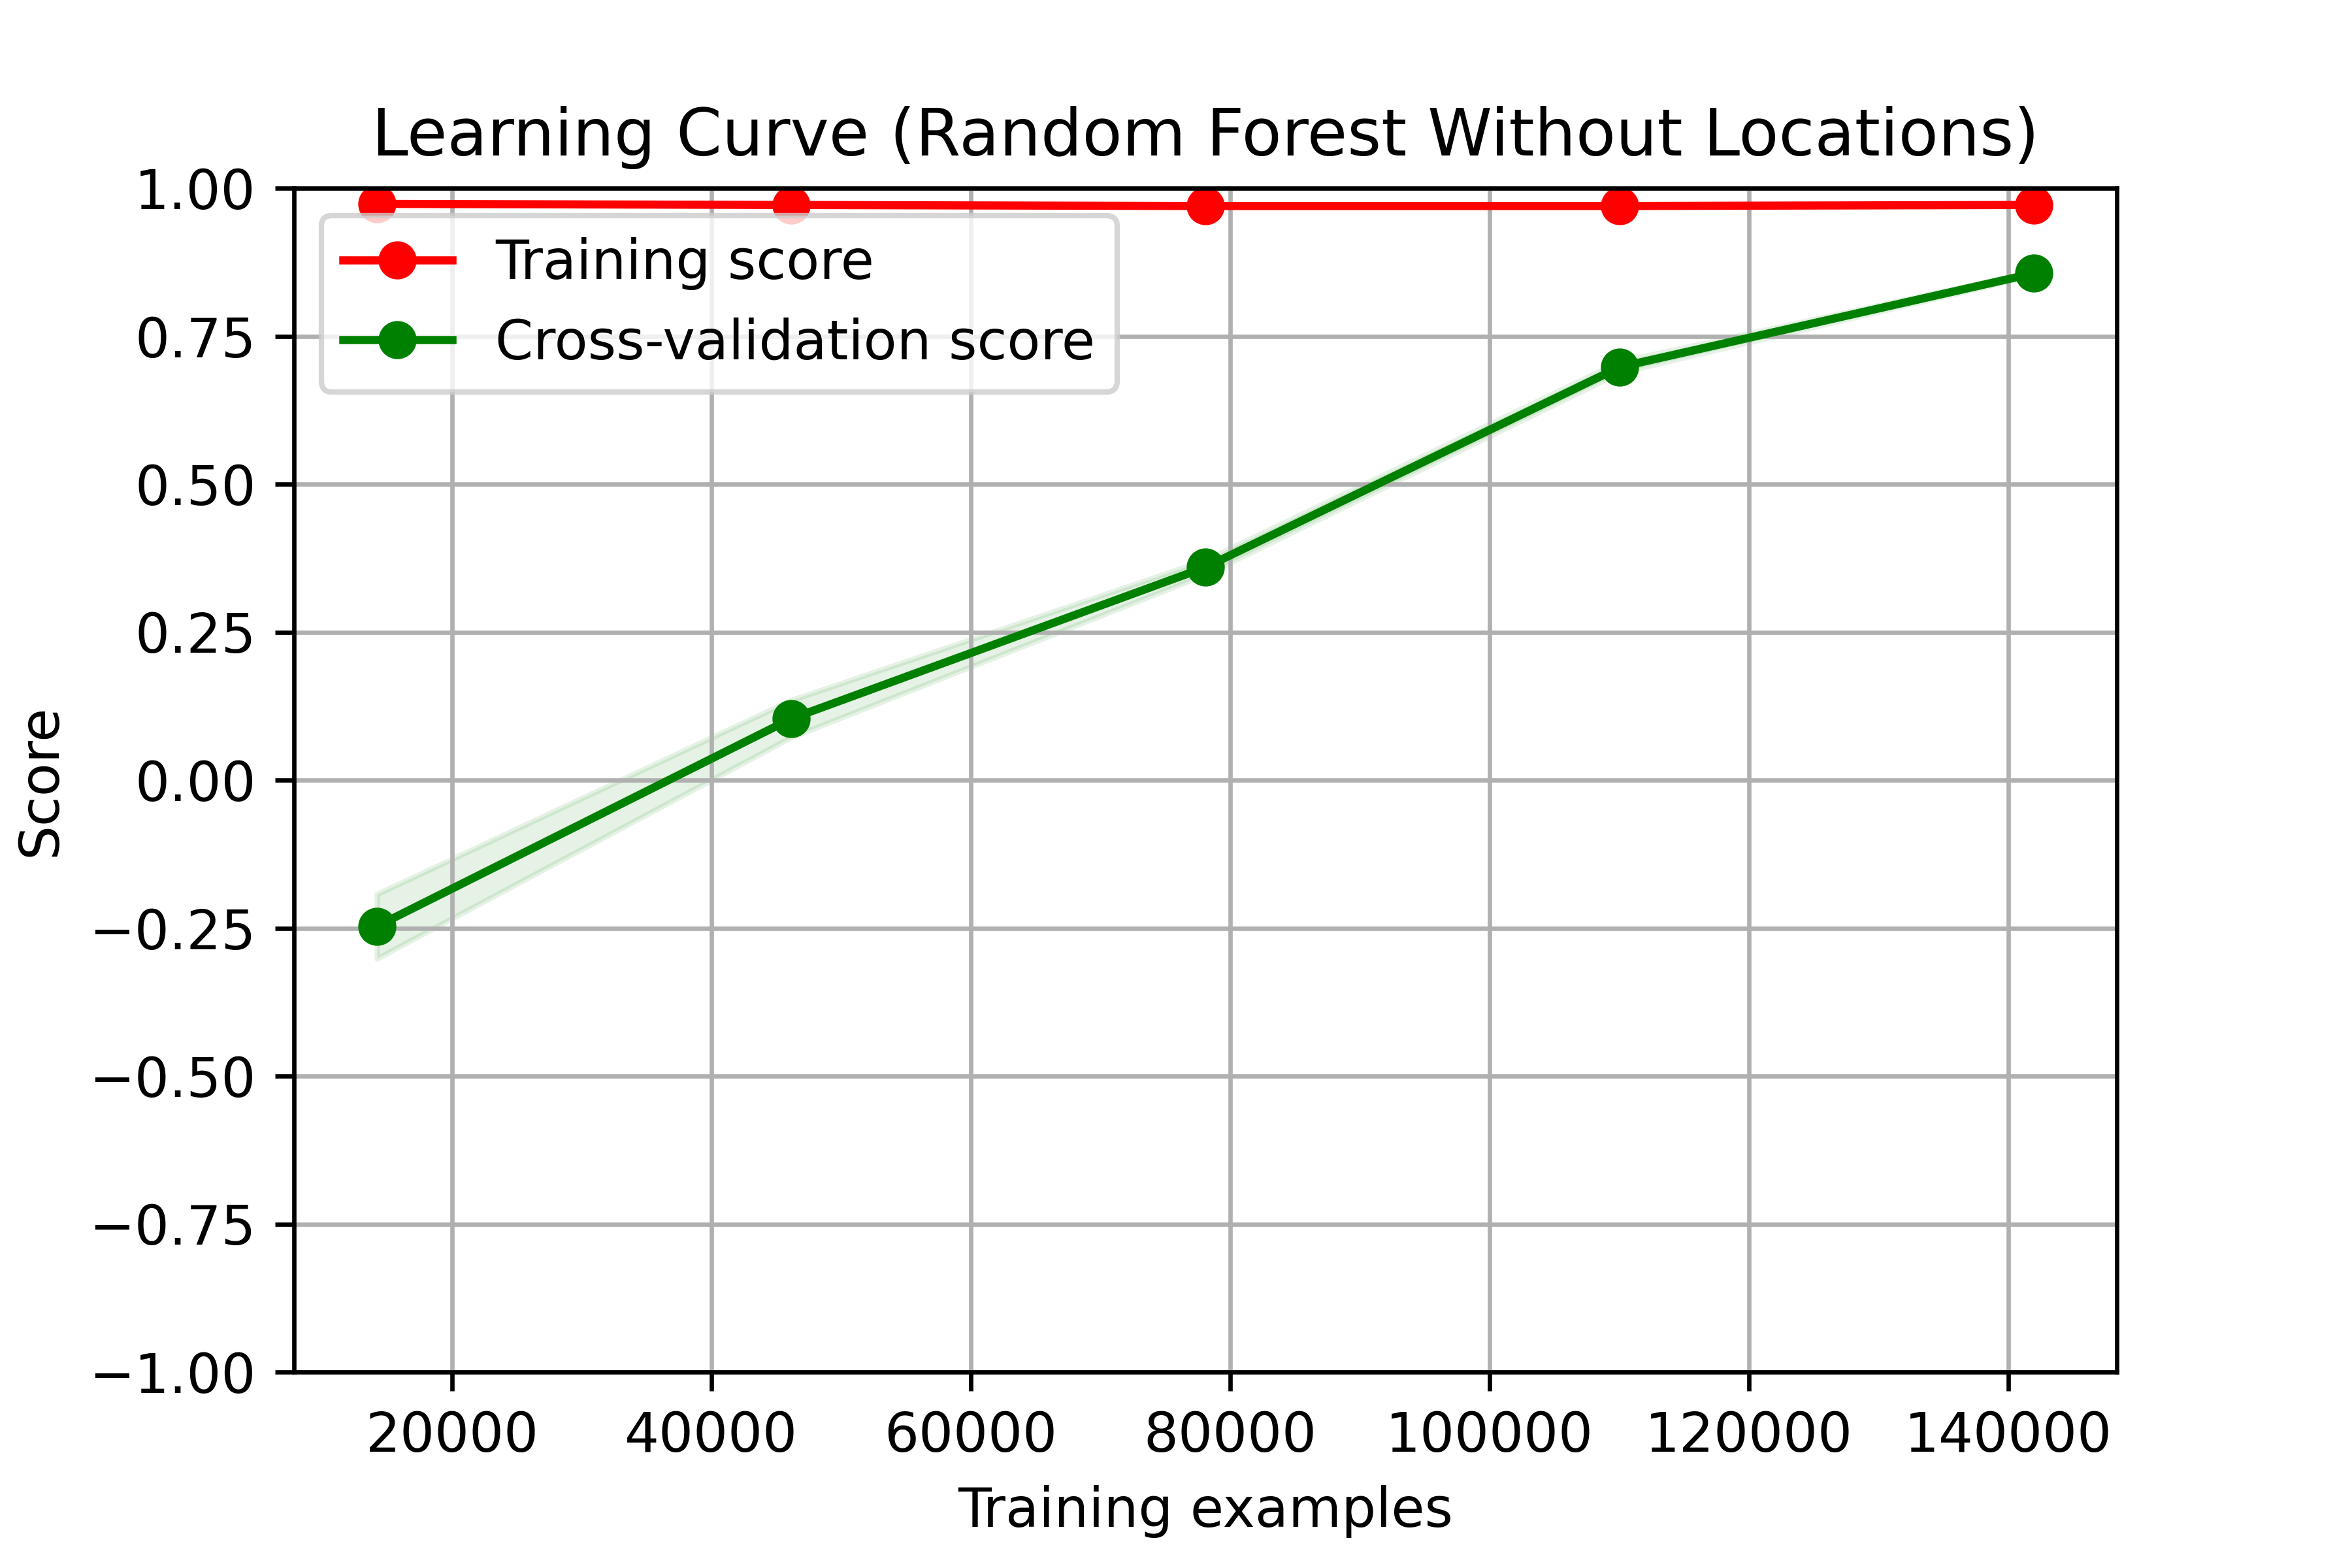
\includegraphics[width=0.5\linewidth]{./figures/Learing Curve1.png}}
\subfloat[\label{cv2}]{%
      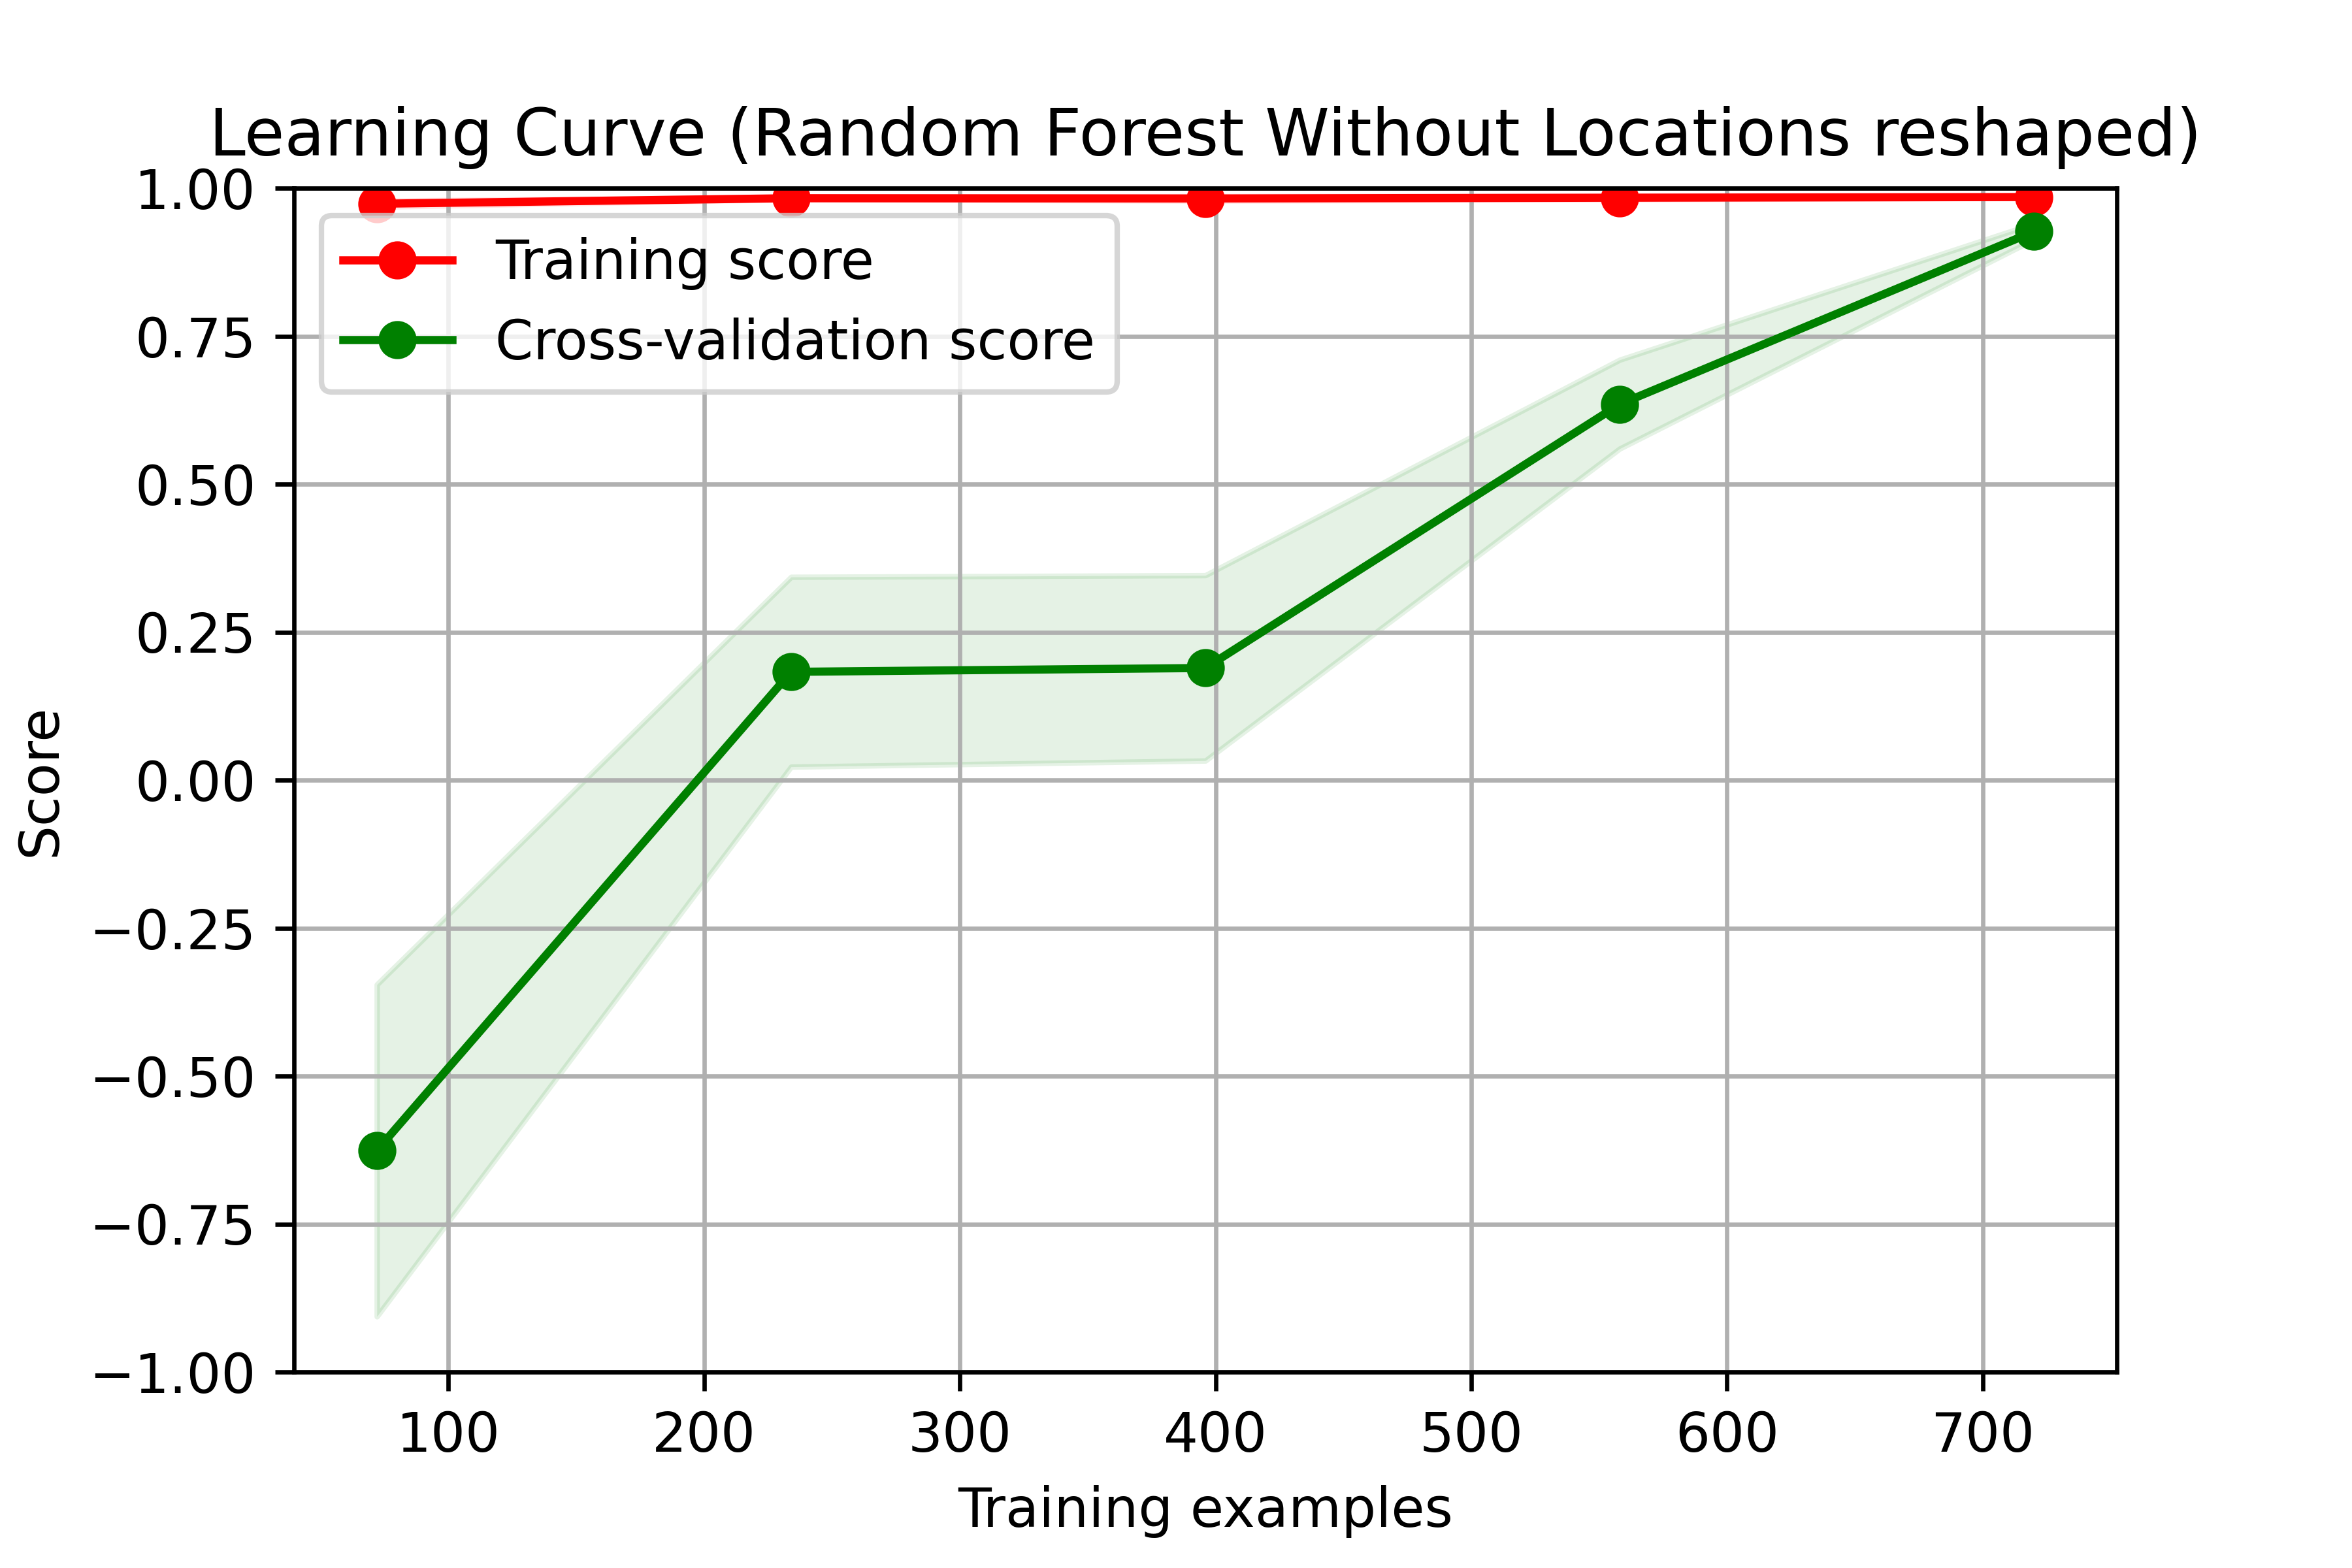
\includegraphics[width=0.5\linewidth]{./figures/Learing Curve2.png}}
\hfill
\subfloat[\label{cv3}]{%
      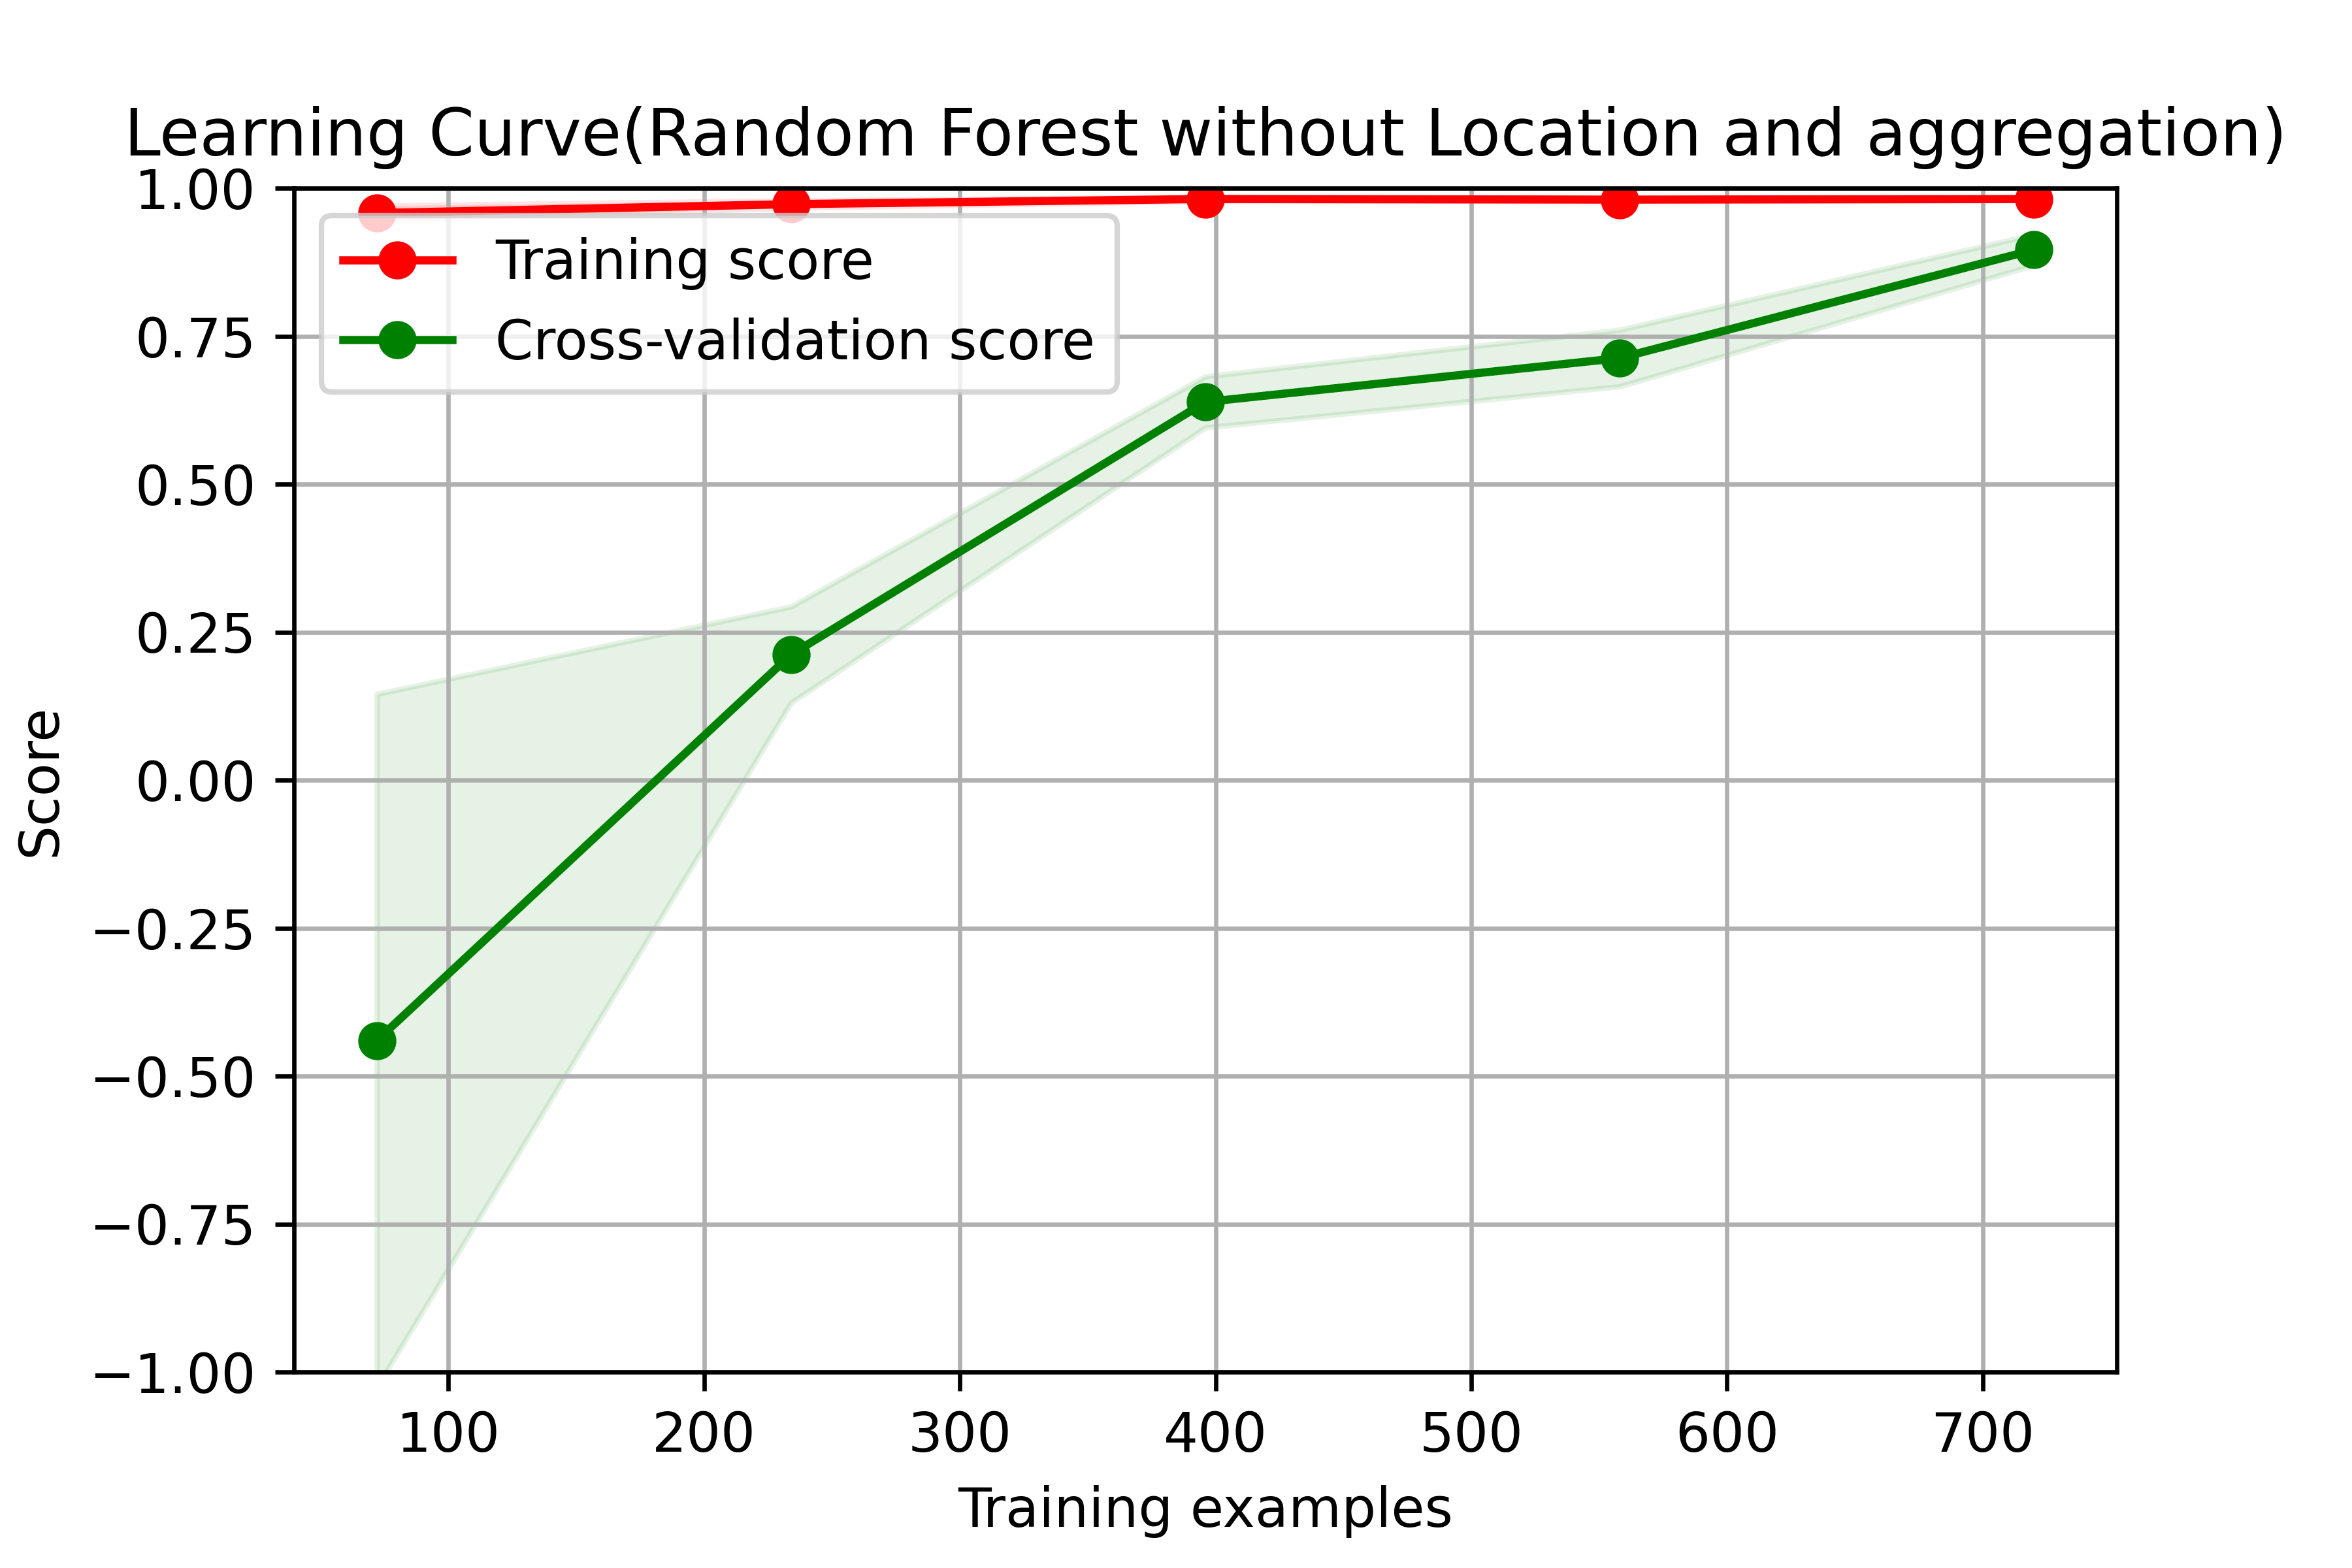
\includegraphics[width=0.5\linewidth]{./figures/Learning Curve(Random Forest without Location and aggregation).png}}
\subfloat[\label{cv4}]{%
      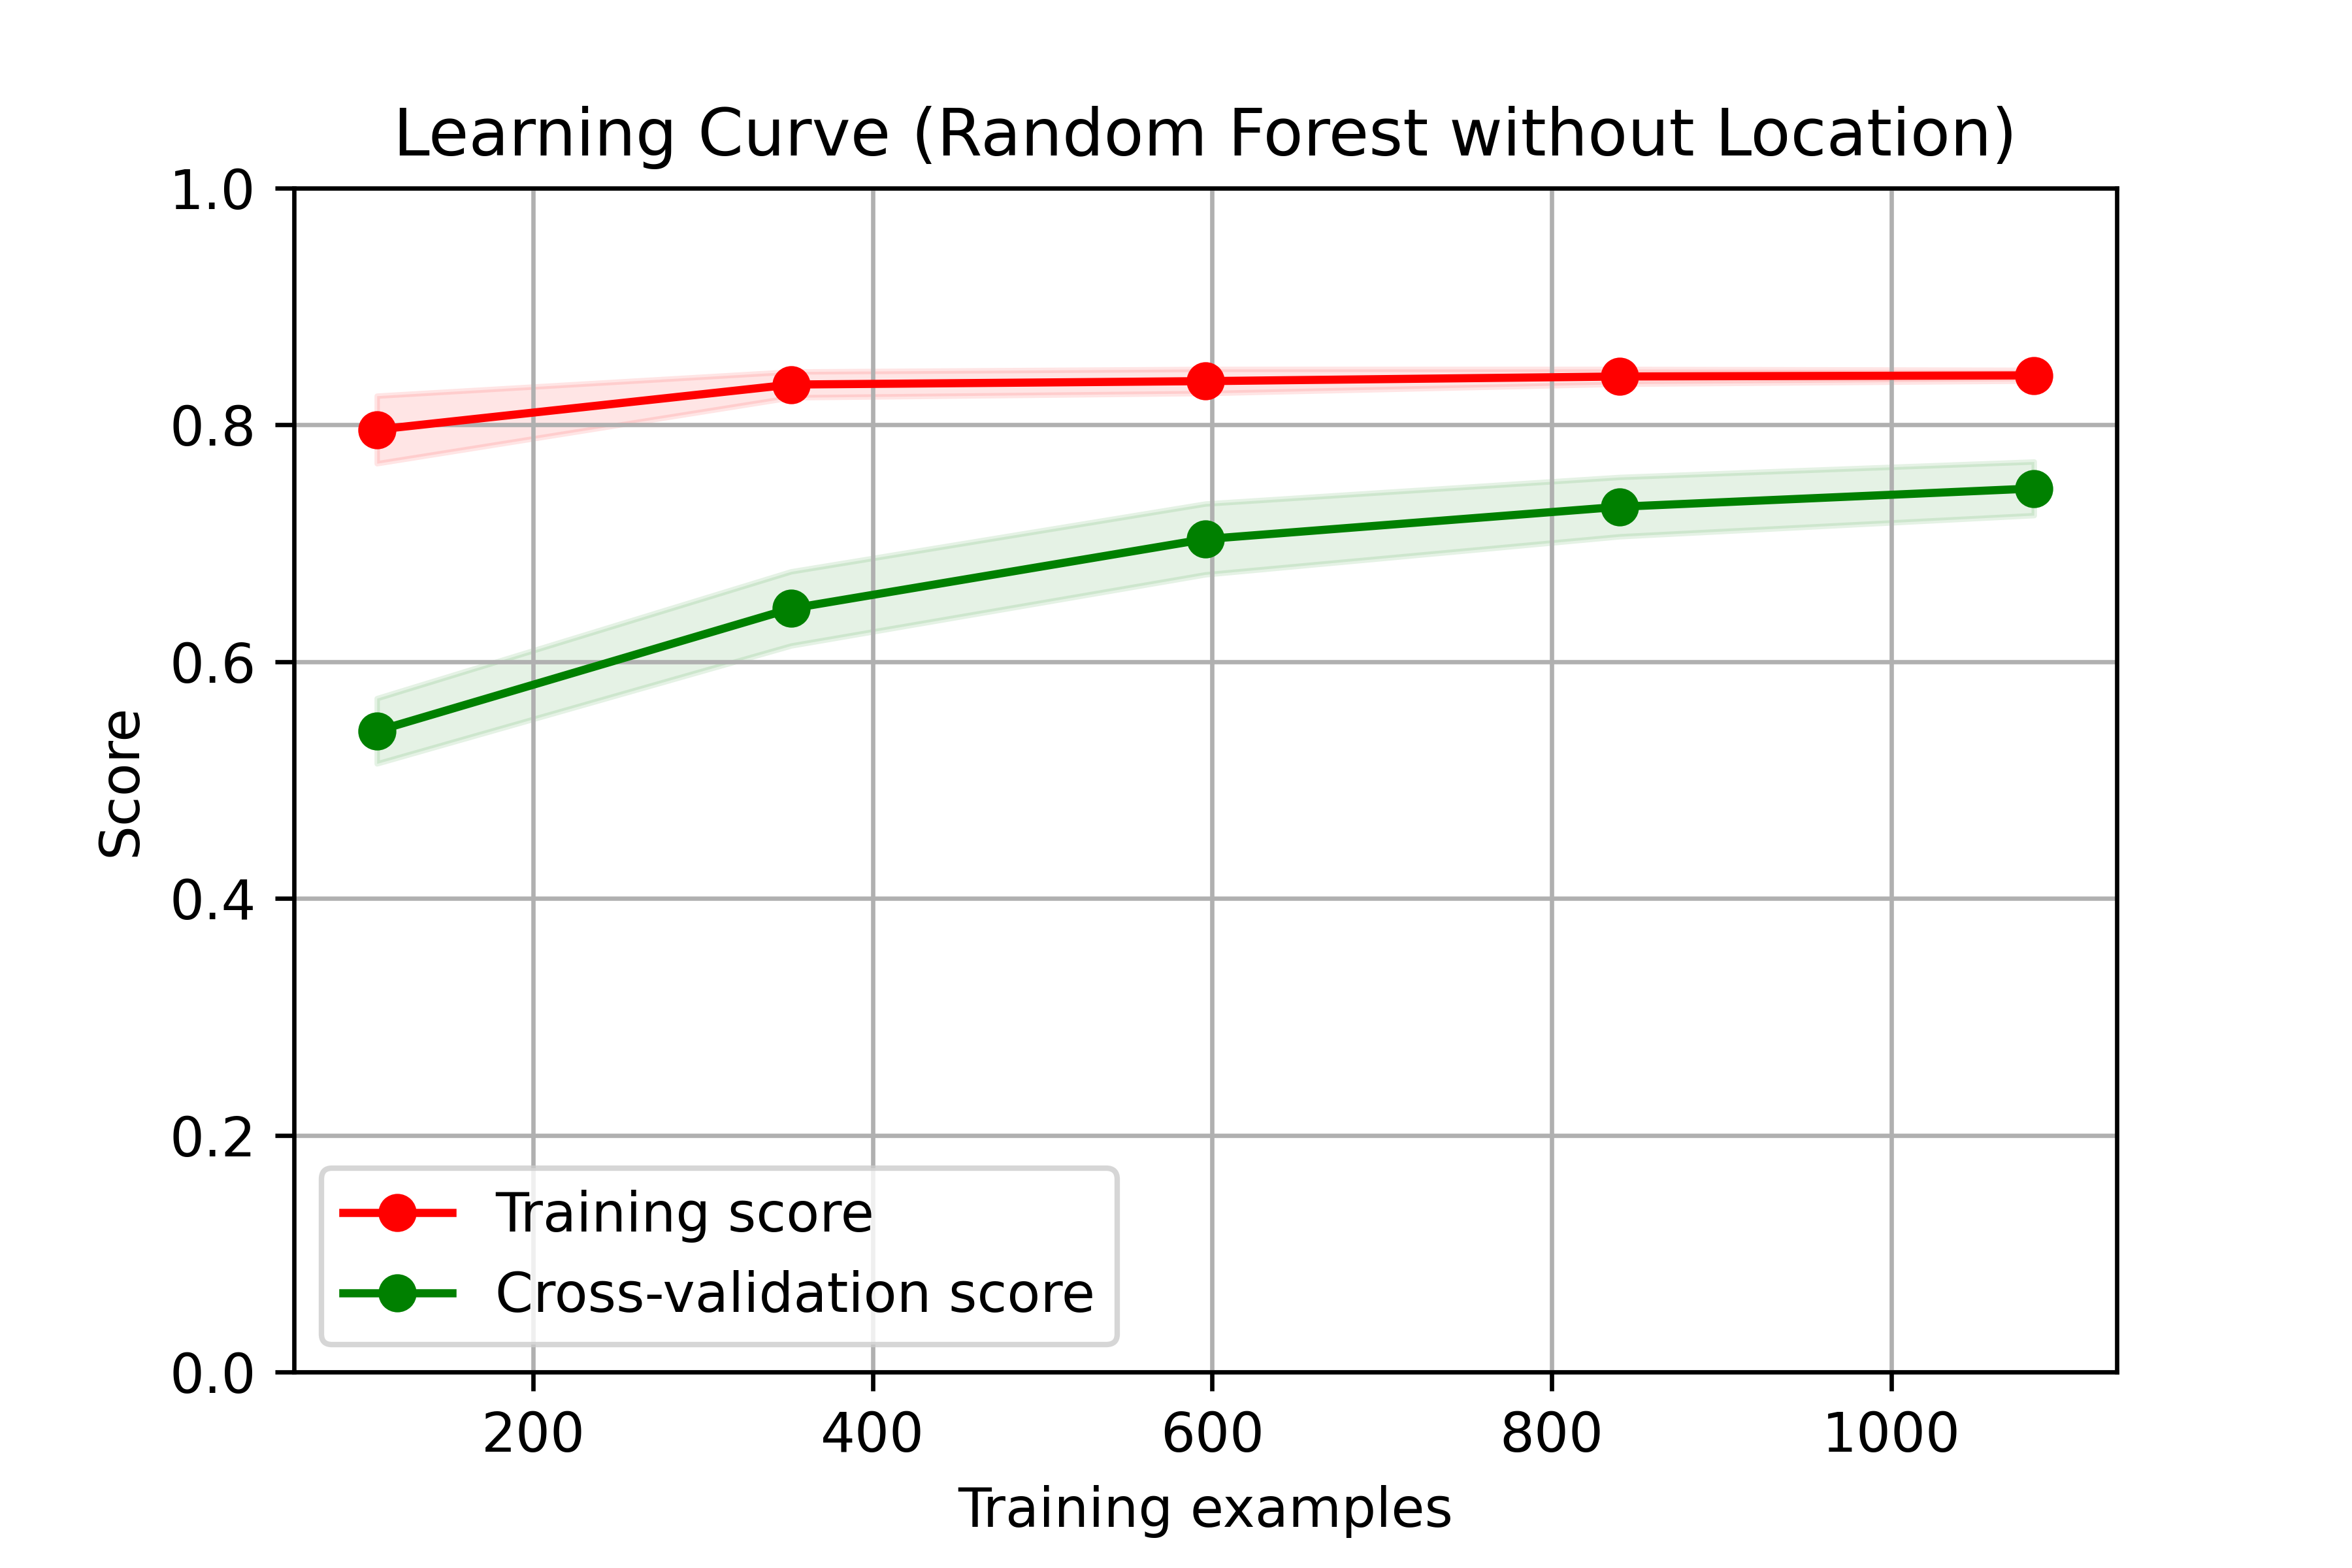
\includegraphics[width=0.5\linewidth]{./figures/cv4.png}}
\label{fig:lc} 
\caption{Learning Curve}
\end{figure}

Reshape data to shrink the disparity between yield and data entries. For data in 2013, the origin shape is $(166685,16)$, means that there are 186 days every location for 16 features. Transform the shape of data in to $(901\times2960)$ and run test again get the learning curve shown in Fig.~\ref{cv2}. These two methods can't solve the overfitting problem.

Try to aggregate the data to shrink the number of features. Calculate the mean values of ever 60 days and shrink features to 48, run test again and get the learning curve shown in Fig.~\ref{cv3}. There are some improvement after half of the dataset geting involved.

Extract some indirect features from the origin features, calculate the minimum and maximum value of features in 30 days, minimum maximum NDVI in 30 days, mean temperature difference and variance e.t using rolling window method from pandas. Then, run test base on these indirect features get the learning curve in Fig.~\ref{cv4}.

\subsection{LSTM}
Use EarlyStopping callback function to alleviate overfiting and set training epoch to 1000. The process of training shown in %Fig.~\ref{fig:train}.

\begin{figure*}[htbp]
  \centerline{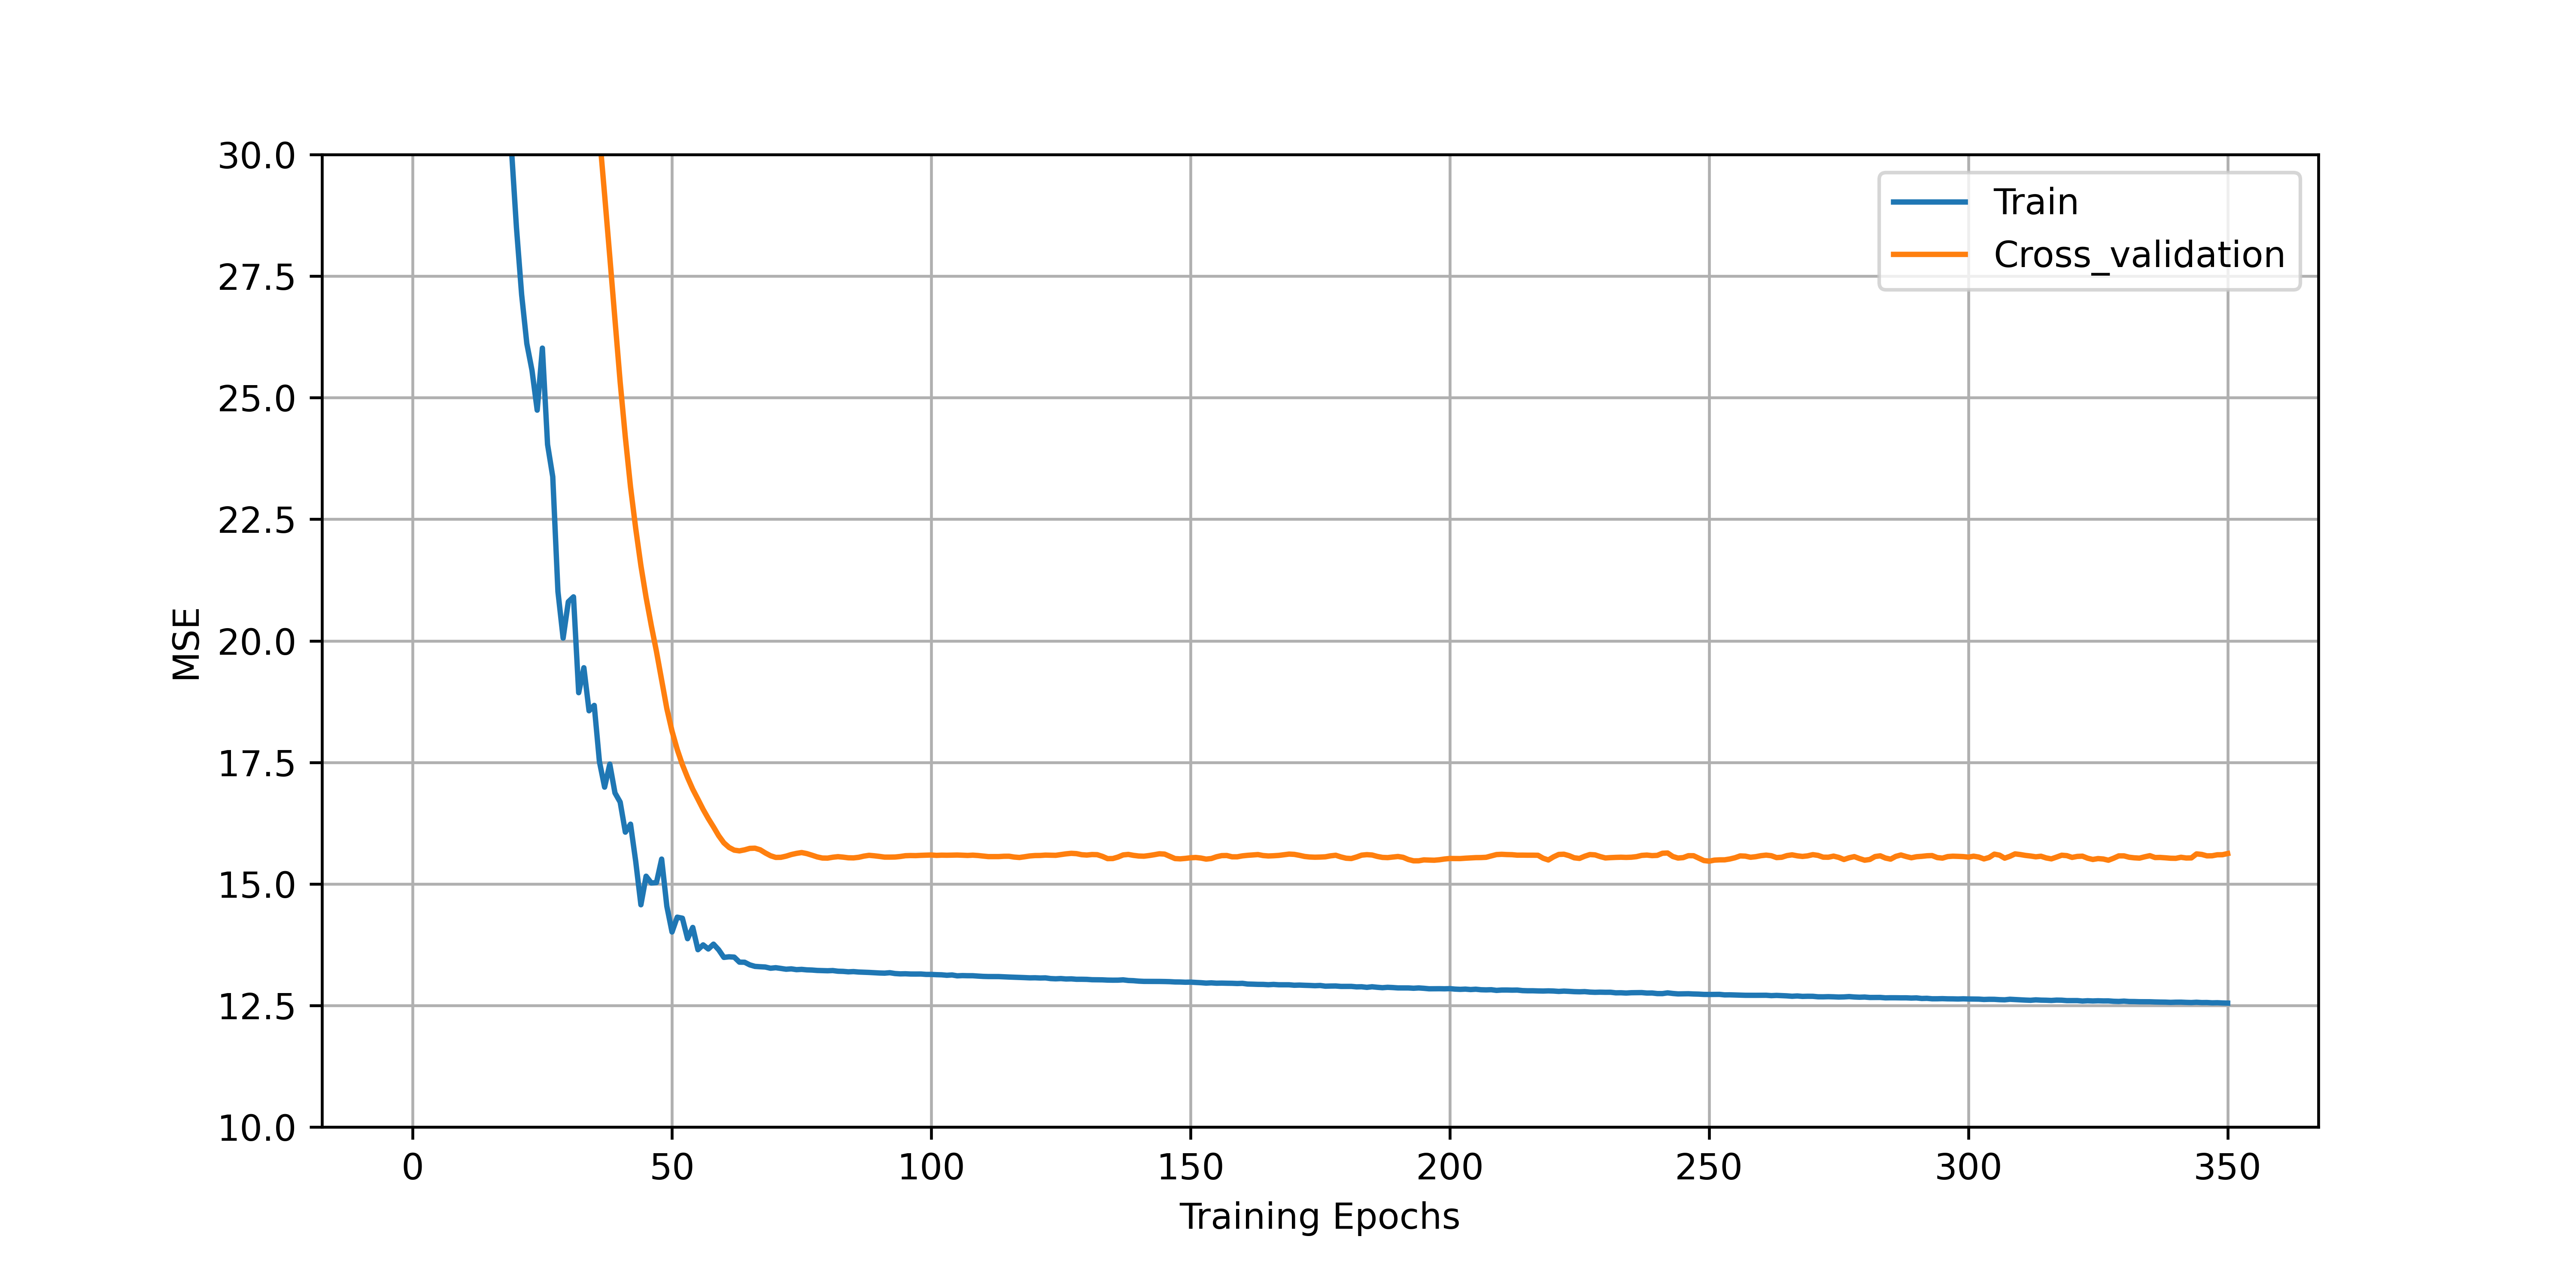
\includegraphics[width=\linewidth]{figures/lp.png}}
  \caption{Training Process of LSTM}
  \label{fig:train}
\end{figure*}

The MSE of both training and cross validation go lower acompanied with the incresment of taining epochs. This procedure has been run several times, it always triggers the EarlyStopping callback function at between 100 to 300 epochs. The final mean cross validation MSE for all runs is 12.3793 comparing to RF's 23.72, the performance of LSTM is 47.84\% better than RF which is quite accurate to forecast the yield of corps whose $R^2$ error is 83.61\% after solving the overfitting problem.

\section{Conclusion} \label{sec:con}
It is found that both LSTM and RF algorithm do well in prediction of agricultural production, but there are some difference between them.

The implementation of LSTM is more comlpex, and many parameters need to be test and decided, and it is not easy to change the data's structure when there are new data get involved. There will be more time needed to config the model to meet the change of data either on features or recorded days. What's more, the training of a neural network consumes a lot of computing resources comparing to random forest. The random forest, on the contrary, less work needed to fit the change of data but more work needed to get pretreatment data, which alleviate the overfitting problem.

\section{Future work} \label{sec:fw}
Some features which are crucial to the growing of crops, such as how farmers plant the crop, the condition of sow in a certain location e.t, are not involved to the models due to the lack of data source. The weather, undoubtedly, can influence the yield of corps, but some subjective behaviors can greatly improve the yield. The corps are not planted in an environment free of human intervention, water the crops when precipitation is in a low level is a natural behavior. If can get access such sort of data , the accuracy of prediction will be higher. 

\bibliographystyle{IEEEtran}
\bibliography{IEEEabrv,reference}

\end{document}
